\documentclass[a4paper,11pt]{report}
\usepackage{amsmath}
\usepackage{graphicx}
\usepackage{wrapfig}
\usepackage{caption}
\usepackage{enumitem}
\usepackage{pdfpages}
\usepackage{multicol}
\usepackage[a4paper, left=3cm, right=3cm, top=3cm, bottom=3cm]{geometry}
\usepackage[ngerman]{babel}
\usepackage{hyperref}
\usepackage[x11names]{xcolor}
\usepackage{fancyhdr}
\pagestyle{fancy}
\usepackage{tikz}
\usetikzlibrary{calc}
\usepackage{titling}
\usepackage{fontspec}
\usepackage{titlesec}
\usepackage{moresize}
\usetikzlibrary{circuits.ee.IEC}

% font setup
\newfontfamily{\newUpperTitleFont}{Bebas Neue}
\newfontfamily{\newLowerTitleFont}{Tex Gyre Heros Bold}

% font init
\titleformat{\part}[display]{\centering\HUGE\scshape\newUpperTitleFont\color{SlateBlue4}}{\partname~\thepart}{10pt}{}
\titleformat{\chapter}{\Huge\bfseries\newUpperTitleFont\color{SlateBlue4}}{\thechapter}{1em}{}
\titleformat*{\section}{\Large\bfseries\newLowerTitleFont\color{SlateBlue3}}
\titleformat*{\subsection}{\large\bfseries\newLowerTitleFont\color{SlateBlue2}}
\titleformat*{\subsubsection}{\bfseries\newLowerTitleFont\color{SlateBlue1}}

% hyperlink setup
\hypersetup{
    colorlinks,
    citecolor=black,
    filecolor=black,
    linkcolor=SlateBlue3,
    urlcolor=black
}

% clear Footer
\fancyfoot{}

% Header
\fancyhead[L]{A. Lerjen, C. Brülisauer, \\ N. Rahm, N. Fister}
\fancyhead[C]{Kantonsschule - Physik}
\fancyhead[R]{\thepage}
\renewcommand{\headrulewidth}{1pt}
\setlength{\headheight}{30pt}

\fancypagestyle{plain}{
    \fancyhead[L]{A. Lerjen, C. Brülisauer, \\ N. Rahm, N. Fister}
    \fancyhead[C]{Kantonsschule - Physik}
    \fancyhead[R]{\thepage}
    \renewcommand{\headrulewidth}{1pt}
}

% Title
\title{\Huge\textbf{Bericht Physik - Lautsprecher}}
\author{Andrin Tim Lerjen, Cyrill Brülisauer, Nadja Rahm \& Niklas Fister}
\date{Freitag, 7. März 2025}

% makeing title
\begin{document}
\pagenumbering{Roman}

% pretitle
%
\includepdf[scale=1.05]{resources/pdf/Title.pdf}

% own title
\begin{titlepage}
    \centering
    \begin{tikzpicture}[remember picture, overlay]
        \draw[line width=5pt, line cap=round, color=SlateBlue1, rounded corners=5pt]($(current page.west)+(1cm, 0)$) -- ($(current page.north west)+(1cm, -1cm)$) -- ($(current page.north)+(0, -1cm)$);
        \draw[line width=5pt, line cap=round, color=SlateBlue1, rounded corners=5pt]($(current page.east)+(-1cm, 0)$) -- ($(current page.south east)+(-1cm, 1cm)$) -- ($(current page.south)+(0, 1cm)$);
    \end{tikzpicture}

    % background
    \tikz[remember picture,overlay] \node[opacity=0.3,inner sep=0pt] at (current page.center){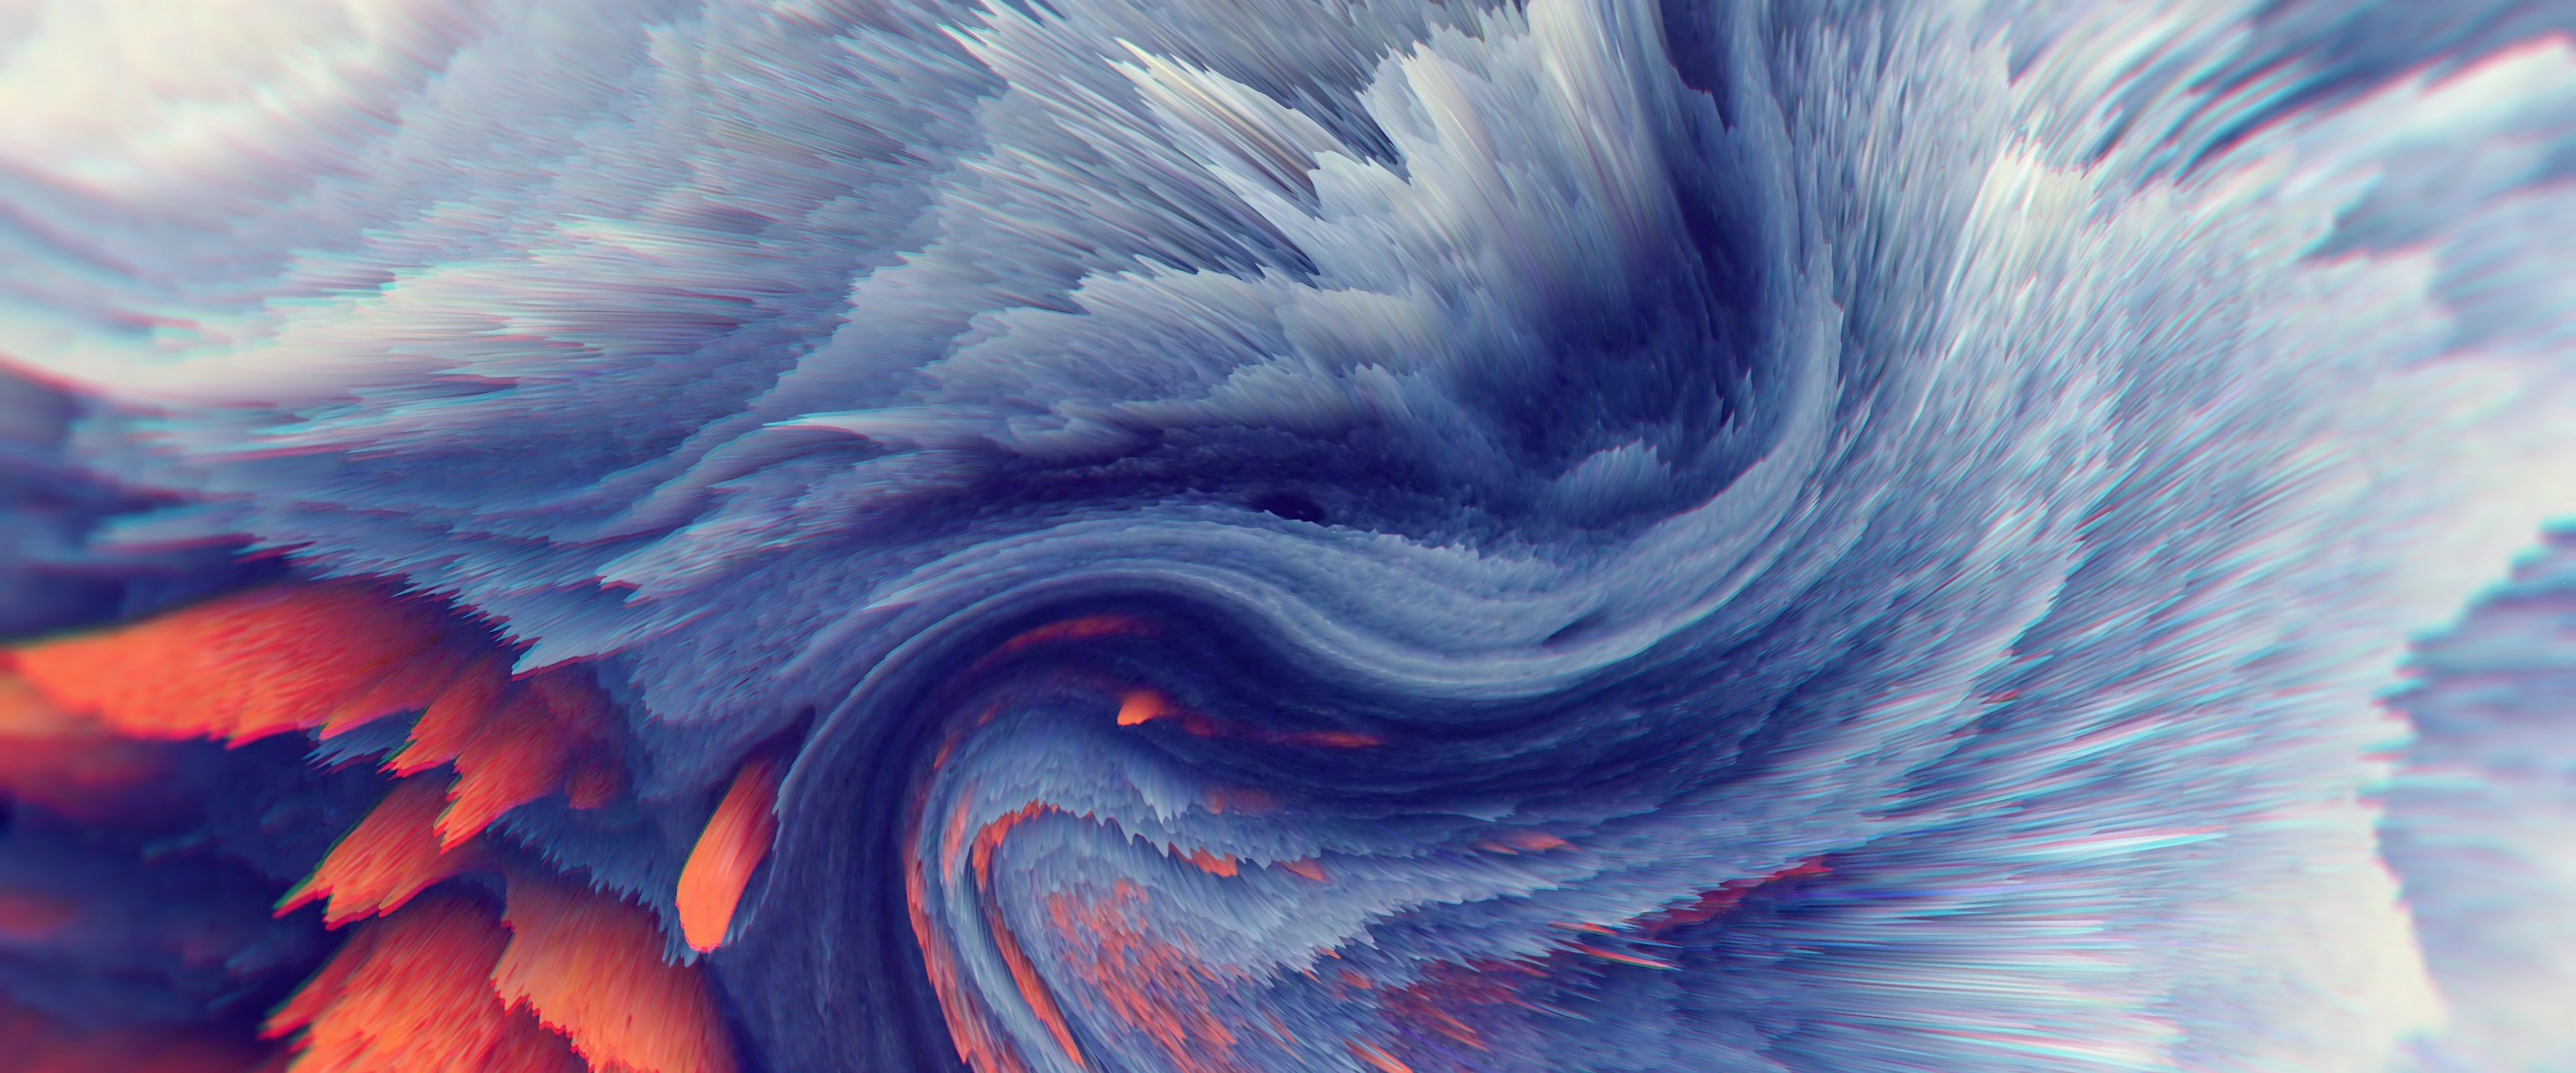
\includegraphics[width=\paperwidth - 4cm, height=\paperheight - 4cm]{resources/images/soundwave.jpg}};
    % Start Text
    \vspace{4cm}

    % the title
    {\newUpperTitleFont\thetitle\par}
    \vspace{1cm}

    % the autors
    {\theauthor\par}
    \vspace{.5cm}

    % date
    {\thedate\par}
    \vspace{5cm}

    % showcase
    %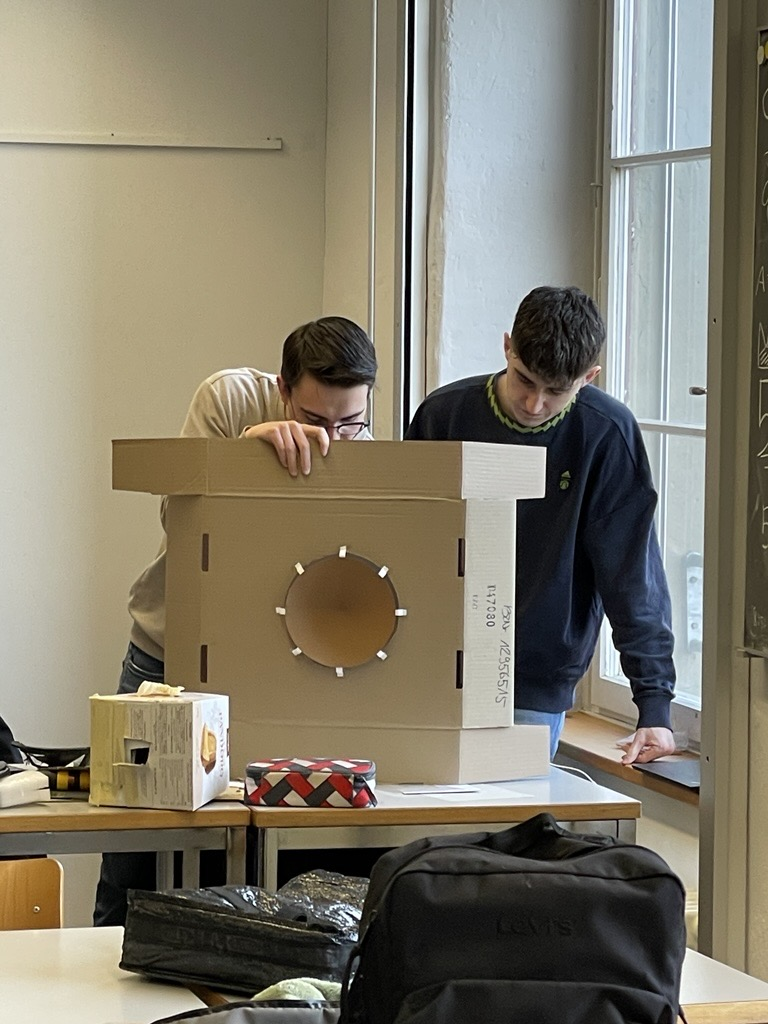
\includegraphics[width=.4\linewidth]{resources/images/Andrin_Cyrill_building.jpeg}
\end{titlepage}

% normal title
%\maketitle

% Abstract
\begin{abstract}
    In dem folgenden Bericht geht es um den Bau eines Lautsprechers aus alltäglichen Materialien.

    Das erzielte Resultat war ein leistungstarker Schallerzeuger, bestehend aus einem Hochtöner und einem Tieftöner, welcher sich vorallem durch seine hochwertige Klangqualität auszeichnet.

    Das gute Klangerlebnis konnte vorallem durch eine präzise Bauweise und gutes Prototyping erreicht werden.
\end{abstract}

% Table of contents
\tableofcontents
\thispagestyle{empty}

% report
\pagenumbering{arabic}
\setcounter{page}{1}

% Bericht
\part{Bericht}

% Introduction
\chapter{Einleitung}
\section{Aufgabestellung}
Die Aufgabe war es, einen Lautsprecher aus Haushaltsmaterialien zu bauen, welcher in drei Kategorien möglichst gut abschneitet. Die bewerteten Kriterien lauten wie folgt:
\begin{itemize}
    \item \textbf{Klangqualität:} Höhen, Bässe, Lautstärke bis Scheppern oder Vibra eingesetzt
    \item \textbf{Lautsprecherdesign:} Ästhetik, Originalität, Komfort
    \item \textbf{Baudokumentation:} Verständlichkeit, Informationstiefe, Layout 
\end{itemize}
\section{Umsetzung}
Die Gruppe hat sich dafür entschieden, den Fokus primär auf die Klangqualität zu richten. Somit lag das Design an zweiter Stelle, sollte jedoch auch berücksichtigt werden. Dies sollte dafür sorgen, dass genügend Zeit für Versuche geschaffen wird, welche das erreichen der maximalmöglichen Klangqualität ermöglichen.

\newpage
\section{Theorie}
\subsection{Grundlegende Formeln}
\textbf{Relevante Variablen} \par
\begin{tabbing}
    gamma\quad\= a Greek latter\kill
    \(\mu_0\) :     \> magnetische Permeabilität des Vakuums \\
    \(\mu_r\) :     \>magnetische Permeabilität des Füllmaterials \\
    \(N\) :         \> Anzahl Windungen \\
    \(I\) :         \>Stromstärke \\
    \(L\) :         \>Länge der Spule \\
\end{tabbing}

\textbf{Berechnung der magnetischen Permeabilit im Vakuum}
\begin{equation}
    \mu_0 = 4 \cdot \pi \cdot 10^{-7} \frac{V \cdot s}{A \cdot m}
\end{equation}\par

\textbf{Berechnung der magnetischen Kraft mit Füllmaterial}
\begin{equation}
    B(r) \approx \frac{\mu_0 \cdot \mu_r \cdot N \cdot I}{L}
\end{equation}\par

\subsection{Geschichte des Lautsprechers}

\begin{wrapfigure}{r}{0.4\textwidth}
    \centering
    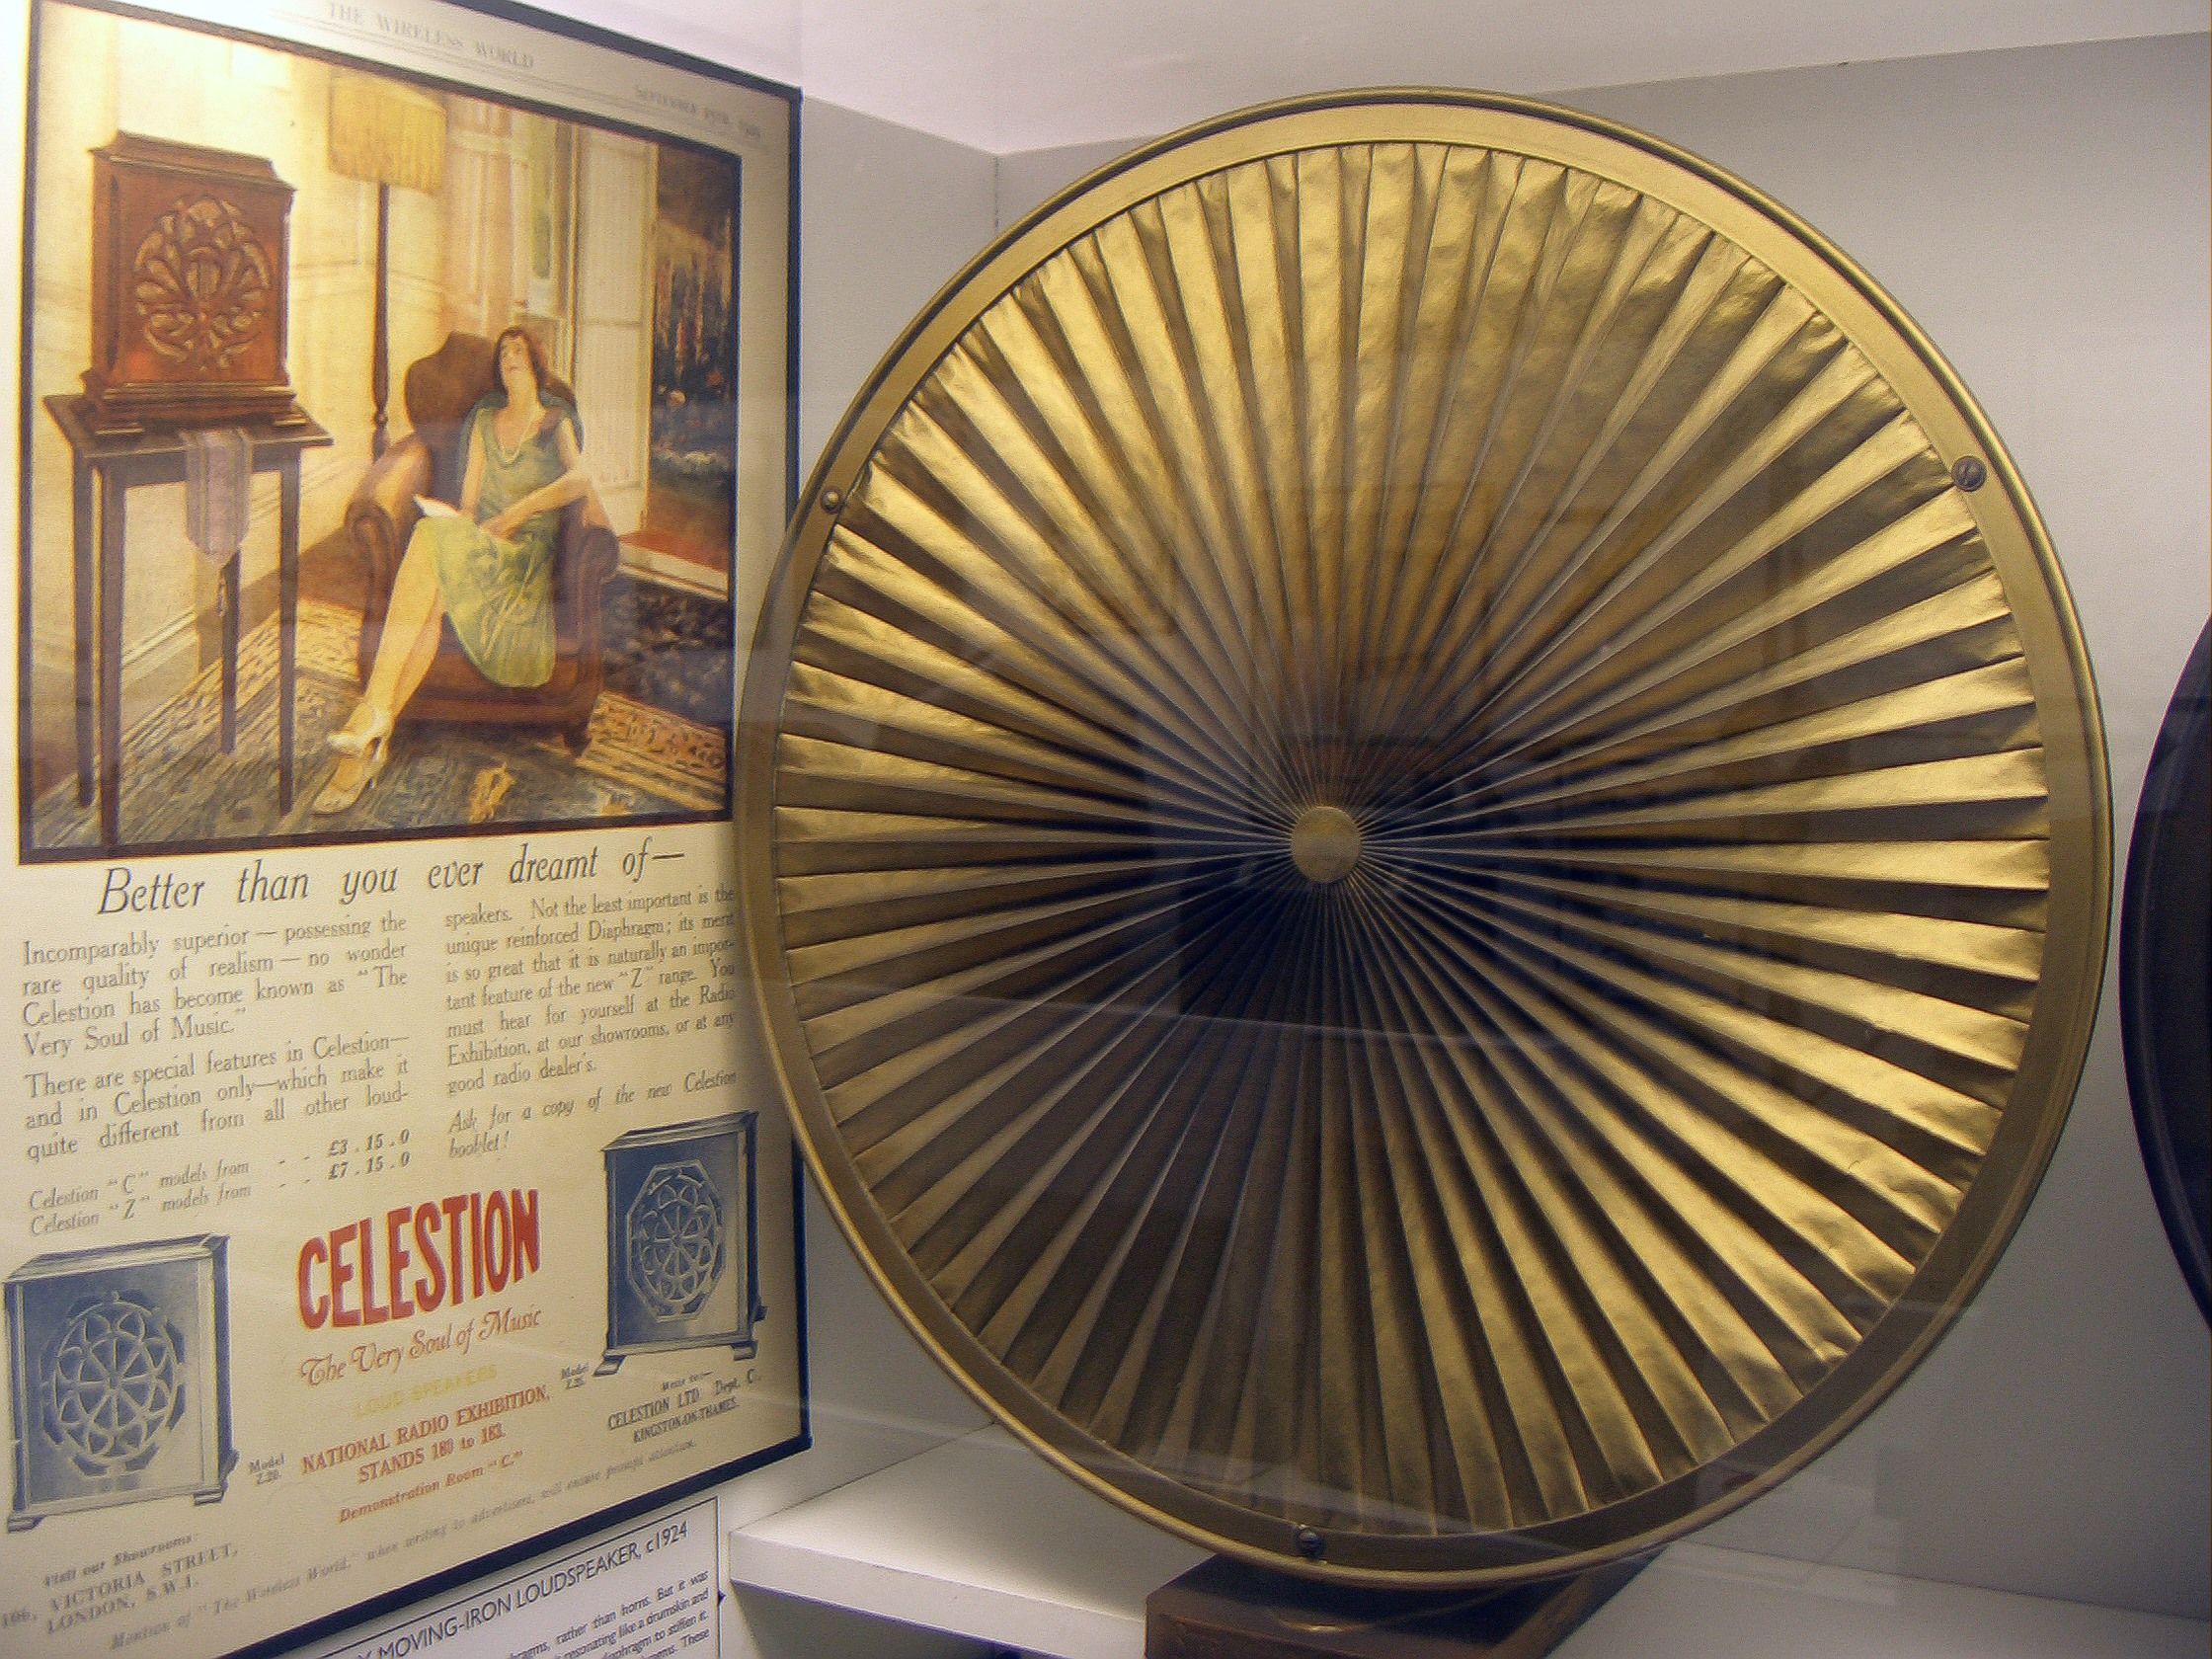
\includegraphics[width=.95\linewidth]{resources/images/Lautsprecher_Celestion.jpg}
    \caption{\raggedright{Lautsprecher von Celestion}}
    \label{fig:celection_speaker}
\end{wrapfigure}

Der Lautsprecher wurde im Jahre 1861 als mechanisches Nebenprodukt des Telefons entwickelt.

1878 wurde dann das Patent zu einem elektrischen Lautsprecher eingereicht, welches letztlich erst 1925 präsentiert wurde.
Das Grundprinzip blieb bis heute unverändert und ist in den meisten Lautsprechern vorzufinden. \cite{history_wikipedia}

Aufgrund der damaligen Bauweise der leichten, weich eingespannten Membran waren die Lautsprecher meinst sehr gross.\cite{history_connect}

Einen Entwickler für den Lautsprecher kann man jedoch nicht genau nennen, da es eine fliessende Entwicklung war, welche schlussendlich zum Lautsprecher wie man ihn heute kennt führten.

Viele forschten gleichzeitig an diesem Thema und Patente unterschieden sich nur vage. Teils waren die Patente in den USA und Deutschland sogar nahezu identisch.\cite{history_tu_berlin}

% How to build it properly
\newpage
\subsection{Ideale Bauweise}
\subsubsection*{Bassreflexgeäuse}
\vspace{.5cm}
\noindent \begin{minipage}{0.6\textwidth}
    Um eine möglichst gute Basswiedergabe zu generieren, ist die Bauart eines Bassreflexgehäuses optimal. Ermöglicht wird dies durch die offene Gehäusegestaltung mit einem sogenannten "Bassreflexkanal".
    Das Innere des Körpers fungiert dabei als Resonator, um den Bass zu verstärken.
\end{minipage}
\hspace{0.1\textwidth}
\begin{minipage}{0.2\textwidth}
    \includegraphics[width=.9\textwidth]{resources/images/Bassreflex-Gehäuse.png}
    \captionof{figure}{\raggedright Bassreflex-Gehäuse}
    \label{fig:bass-reflex}
\end{minipage}
\vspace{.5cm}

Dabei wird diese allgemeine Formel für die Berechnung von Resonatorkanäle mit kreisförmigen Querschnitt verwendet:
\begin{tabbing}
    gamma\quad\= a Greek latter\kill
    d :    \>Durchmesser (in cm) \\
    l :    \>Länge (in cm)
\end{tabbing}

\begin{equation}
    l = \frac{23400 \cdot d^2}{f^2 \cdot V_b} - 0.8 \cdot d
\end{equation}
Diese Bauform ist jedoch vor allem für reine Tieftöner-/Subwooferboxen geeignet.\cite{bassreflex_wikipedia}

\subsubsection*{Frequenzweichen}
Über eine Frequenzweiche ist es möglich das Audiosignal des Verstärkers in seine Höhen und Tiefen (teils auch Mitten) aufzuteilen. Somit können die Höhen an den dafür vorgesehen Hochtöner geleitet werden und die Tiefen an den entsprechenden Tieftöner. Dies verhindert, dass der Hochtöner bei der Wiedergabe von Tiefen zu scheppern beginnt und der Tieftöner die hohen Frequenzen verschwimmen lässt. 

Im Folgenden ist eine Zwei-Wege-Frequenzweiche dargestellt. Die Kondensatoren verringern ihren internen Widerstand mit der steigenden Frequenz. So sorgt dies beim Hochtöner dafür, dass der Strom bei hohen Frequenzen durch dessen Spule geführt wird. Im Gegensatz dazu führt dieser Effekt beim Tieftöner dafür, dass der Strom bei hohen Frequenzen abgeleitet wird. Um die sich dadurch ändernde Impedanz auszugleichen, werden zwei Spulen verwendet. 
\newpage
Das Schema sieht wie folgt aus: \\
\begin{center}
    \begin{tikzpicture}[rotate=-90, circuit ee IEC,x=3cm,y=2cm,semithick,
        every info/.style={font=\footnotesize},
        small circuit symbols,
        set resistor graphic=var resistor IEC graphic,
        set diode graphic=var diode IEC graphic,
        set make contact graphic= var make contact IEC graphic]
    % Let us start with some contacts:
    \foreach \contact/\y in {1/1,2/2,3/3.5,4/4.5}
    {
    \node [contact] (left contact \contact) at (0,\y) {};
    \node [contact] (middle contact \contact) at (1,\y) {};
    \node [contact] (right contact \contact) at (2,\y) {};
    }
    \draw (right contact 1) -- (right contact 2) -- (right contact 3)
    -- (right contact 4);
    
    \draw (left contact 1) to ++(down:1)
             to [ac source] ++(right:2)
             to (right contact 1);
    
    \draw (left contact 1) to (left contact 2);
    \draw (left contact 2) to [inductor] (middle contact 2);
    \draw (middle contact 1) to (middle contact 2);
    \draw (middle contact 1) to [capacitor] (right contact 1);
    \draw (middle contact 2) to [resistor={info={[SlateBlue1]$TT$}}] (right contact 2);
    \draw (left contact 2) to (left contact 3);
    \draw (left contact 3) to (left contact 4);
    \draw (left contact 4) to [capacitor] (middle contact 4);
    \draw (middle contact 3) to (middle contact 4);
    \draw (middle contact 3) to [inductor] (right contact 3);
    \draw (middle contact 4) to [resistor={info={[SlateBlue1]$HT$}}] (right contact 4);
    \end{tikzpicture}
\end{center}

Um für die gewünschte Übergangsfrequenz (Crossover) die passenden Frequenzweichenteile zu finden, wird folgende Formel verwendet:
Die nötige Induktivität der Spulen lässt sich mithilfe der folgenden Formel berechnen: $C = \frac{R}{\omega}$ 
So die Kapazität der Kondensatoren: $L = \frac{1}{\omega \cdot R}$.

Das Spulen nicht immer mit ihrer Induktivität angeschrieben sind, kann die Induktivität durch eine Spannungsmessung bei fliessendem Wechselstrom errechnet werden. Dafür wird folgende Formel verwendet: $U = I \cdot \omega \cdot L$.

\subsubsection*{Hochpassfilter}
Ein Hochpassfilter (Highpassfilter) sorgt dafür, dass tiefe Frequenzen aus einem Audiosignal herausgefiltert werden und lediglich die Höhen in die Lautsprecherspule geführt werden. Er besteht in seiner einfachsten Ausführung lediglich aus einem oder mehreren Kondensatoren. Dabei bestimmt die Kapazität die Eckfrequenz, also der Punkt, ab welchem Tiefen herausgefiltert werden.

\begin{center}
    \begin{tikzpicture}[rotate=-90, circuit ee IEC,x=1.5cm,y=1.5cm,semithick,
        every info/.style={font=\footnotesize},
        small circuit symbols,
        set resistor graphic=var resistor IEC graphic,
        set diode graphic=var diode IEC graphic,
        set make contact graphic= var make contact IEC graphic]
    % Let us start with some contacts:
    \tikzstyle{contact}=[fill=white, inner sep=0pt, outer sep=0pt]
    \tikzstyle{my_point}=[circle, fill=black, inner sep=1.5pt]
    
    \foreach \contact/\y in {1/1,2/2,3/3,4/3.5,5/4,6/5,7/6,8/7,9/8}
    {
    \node [contact] (lane_1 contact \contact) at (0,\y) {};
    \node [contact] (lane_2 contact \contact) at (1,\y) {};
    \node [contact] (lane_3 contact \contact) at (1.5,\y) {};
    \node [contact] (lane_4 contact \contact) at (2.5,\y) {};
    \node [contact] (lane_5 contact \contact) at (3,\y) {};
    \node [contact] (lane_6 contact \contact) at (4,\y) {};
    }
    \draw (lane_3 contact 1) to [ac source] (lane_4 contact 1);
    \draw (lane_3 contact 1) to (lane_3 contact 9);
    \draw (lane_4 contact 1) to (lane_4 contact 4);
    \draw (lane_1 contact 2) to [resistor={info={[SlateBlue1]$TT$}}] (lane_2 contact 2);
    \draw (lane_5 contact 2) to [resistor={info={[SlateBlue1]$HT$}}] (lane_6 contact 2);
    \draw (lane_1 contact 2) to (lane_1 contact 4);
    \draw (lane_2 contact 2) to (lane_2 contact 3);
    \draw (lane_5 contact 2) to (lane_5 contact 3);
    \draw (lane_6 contact 2) to (lane_6 contact 5);
    \draw (lane_1 contact 4) to (lane_4 contact 4);
    \draw (lane_2 contact 3) to (lane_3 contact 3);
    \draw (lane_4 contact 3) to (lane_5 contact 3);
    \draw (lane_6 contact 5) to (lane_4 contact 5);
    \draw (lane_4 contact 5) to [resistor={ohm=7.2}] (lane_4 contact 6);
    \draw (lane_4 contact 6) to (lane_4 contact 9);
    \draw (lane_4 contact 6) to [capacitor={info=$2.2 \mu F$}] (lane_3 contact 6);
    \draw (lane_4 contact 7) to [capacitor={info=$2.2 \mu F$}] (lane_3 contact 7);
    \draw (lane_4 contact 8) to [capacitor={info=$2.2 \mu F$}] (lane_3 contact 8);
    \draw (lane_4 contact 9) to [capacitor={info=$2.2 \mu F$}] (lane_3 contact 9);
    \node [my_point] (point_1 contact) at (2.5,3) {};
    \node [my_point] (point_1 contact) at (1.5,3) {};
    \node [my_point] (point_1 contact) at (2.5,5) {};
    \node [my_point] (point_1 contact) at (1.5,5) {};
    \node [my_point] (point_1 contact) at (2.5,6) {};
    \node [my_point] (point_1 contact) at (1.5,6) {};
    \node [my_point] (point_1 contact) at (2.5,7) {};
    \node [my_point] (point_1 contact) at (1.5,7) {};
    
\end{tikzpicture}
\end{center}

% Materials and Methods
\chapter{Arbeitsprozess}
\section{Material und Überlegungen}
Bei den Materialien gab es spezifische Ansprüche an Robustheit und Hitzebeständigkeit.

Gerade die Spule forderte hohe Hitzebeständigkeit und die Sicke hohe Belastbarkeit des Materials.

Bei den Materialien des Gehäuses wurde auf die Stabilität und akustische Eigenschaften geachtet.

\subsection{Spule}
\subsubsection*{Trägerkonstruktion}

Beim Konstruieren der Spule wurde auf drei grundlegende Aspekte geachtet. Erstens sollte die Spule so Regelmässig wie möglich gewickelt werden um ein möglichst reines Magnetfeld entstehen zu lassen. Weiter war die Hitzebeständigkeit des Trägermatierials sowie die des Klebstoffes ein Problem. Ein Spulenträger aus einem ferromagnetischen Stoff fiel aufgrund der Beeinflussung des Magnetfeldes weg, ein Träger aus anderen Metallen wäre zu träge und könnte so die Klangqualität beeinflussen. Je schwerer die Membran, desto ungenauer kann ihre Schwingung kontrolliert werden. Kunststoff wäre aufgrund der Schmelztemperaturen auch ungeeignet. Somit hat man sich für ein Rohr aus dünner Graupappe entschieden. Da diese nicht schmelzen kann und über eine sehr hohe Entflammungstemperatur aufweist ist diese für diese Anwendung perfekt geeignet. 

\newpage
\subsubsection*{Draht}
\begin{wrapfigure}{r}{0.4\textwidth}
    \centering
    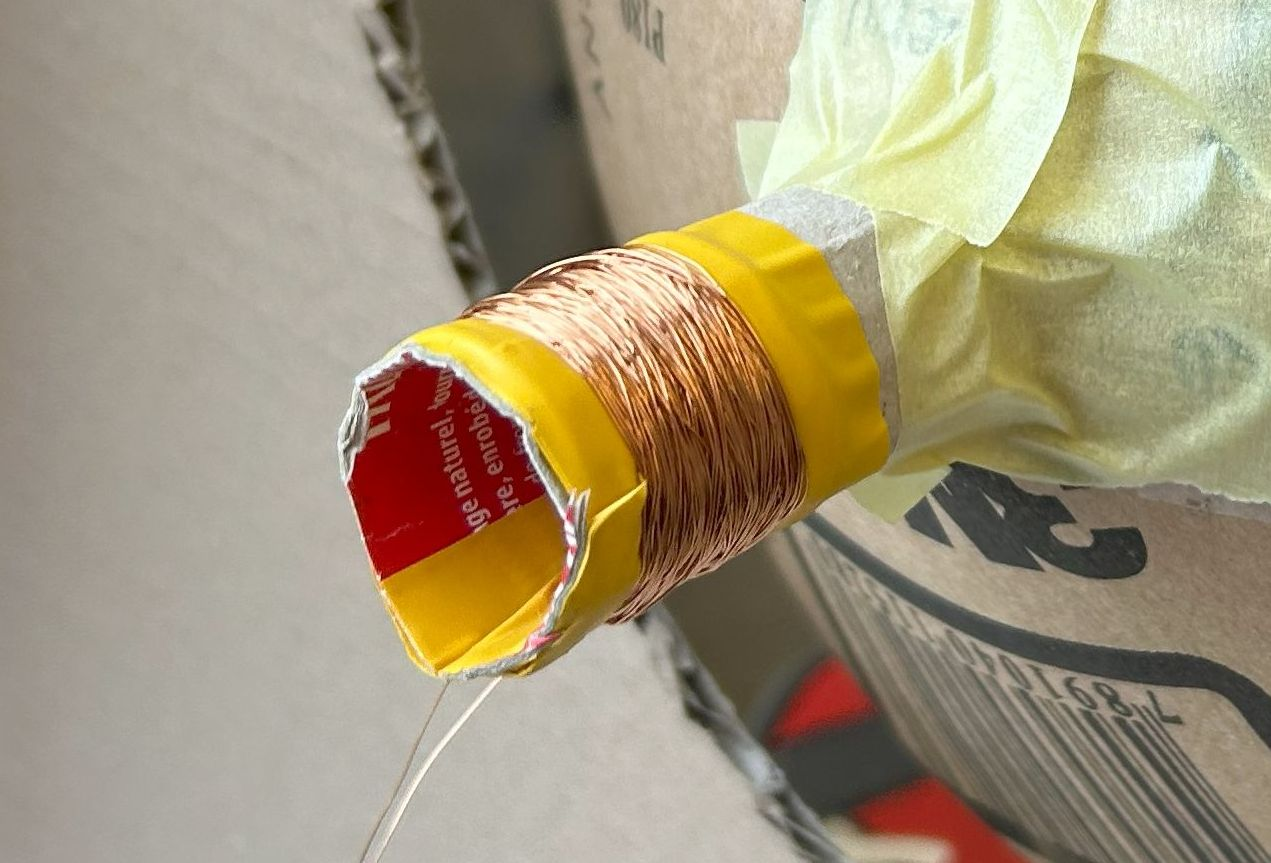
\includegraphics[width=.95\linewidth]{resources/images/Fotos/Physik-62.jpg}
    \caption{\raggedright{Prototyp Spule}}
    \label{fig:spule_prot}
\end{wrapfigure}
Für die eigens durch die Gruppe gewickelte Spule aus Kupferdraht musste die optimale Vorgehensweise ermittelt werden.

Um ein Lösen der Spule zu verhindern, musste diese geleimt werden. Dies geschah mit dem Ofenschnurkleber der Firma Fermit, welcher laut Datenblatt 1100\textdegree C aushalten sollte. Dabei wurden die Klebflächen auf vier Streifen reduziert, um eine bessere Wärmeableitung zu ermöglichen. Die Spule könnte so in der Theorie bis mehrere hundert Grad-Celsius aushalten.  

Nach mehreren Versuchen mit zwei verschiedenen Spulen (siehe Abbildung 2.1) wurde entschieden, dass die optimalsten Spezifikationen für die Spule 400 Wicklungen mit 0,2mm Draht sind. Bei der Hochtönerspule sind es 200 Wicklungen mit 0,2mm Kupferdraht. Der 0,2mm Draht führt zwar zu höheren Widerständen als ein 0,3mm Draht war aber in der verfügbaren Version sehr viel hitzebeständiger. Schlussendlich führte dies zwar zu einer relativ hohen Impedanz von 19,8\Omega\ dafür ist die Spule stark genug um Lautstärken von über 80dB (Abstand 1m) zu erreichen. 

\subsection{Tieftönermembran}
Als Material für die Membran wurde Schleifpapier mit einer Körnung von P180 verwendet. Dieses ist steif genug um sich nicht bei jedem Membranhub zu verformen, aber trotzdem leicht genug um eine flinke Bewegung der Membran zu ermöglichen. Trotzdem ermöglicht der grosse Durchmesser eine Verformung der Membran bei sehr tiefen Frequenzen (<20 Hz) was verhindert das selbst der Maximalhub die Sicke nicht beschädigen kann. Trotzdem ist die Freiheit so beschränkt, dass Frequenzen unter 15Hz nur mit der doppelten Frequenz wiedergegeben werden können. Die fertige Tieftönermembran ist auf der Abbildung 2.2 zu sehen.

\begin{figure}[h]
    \centering
    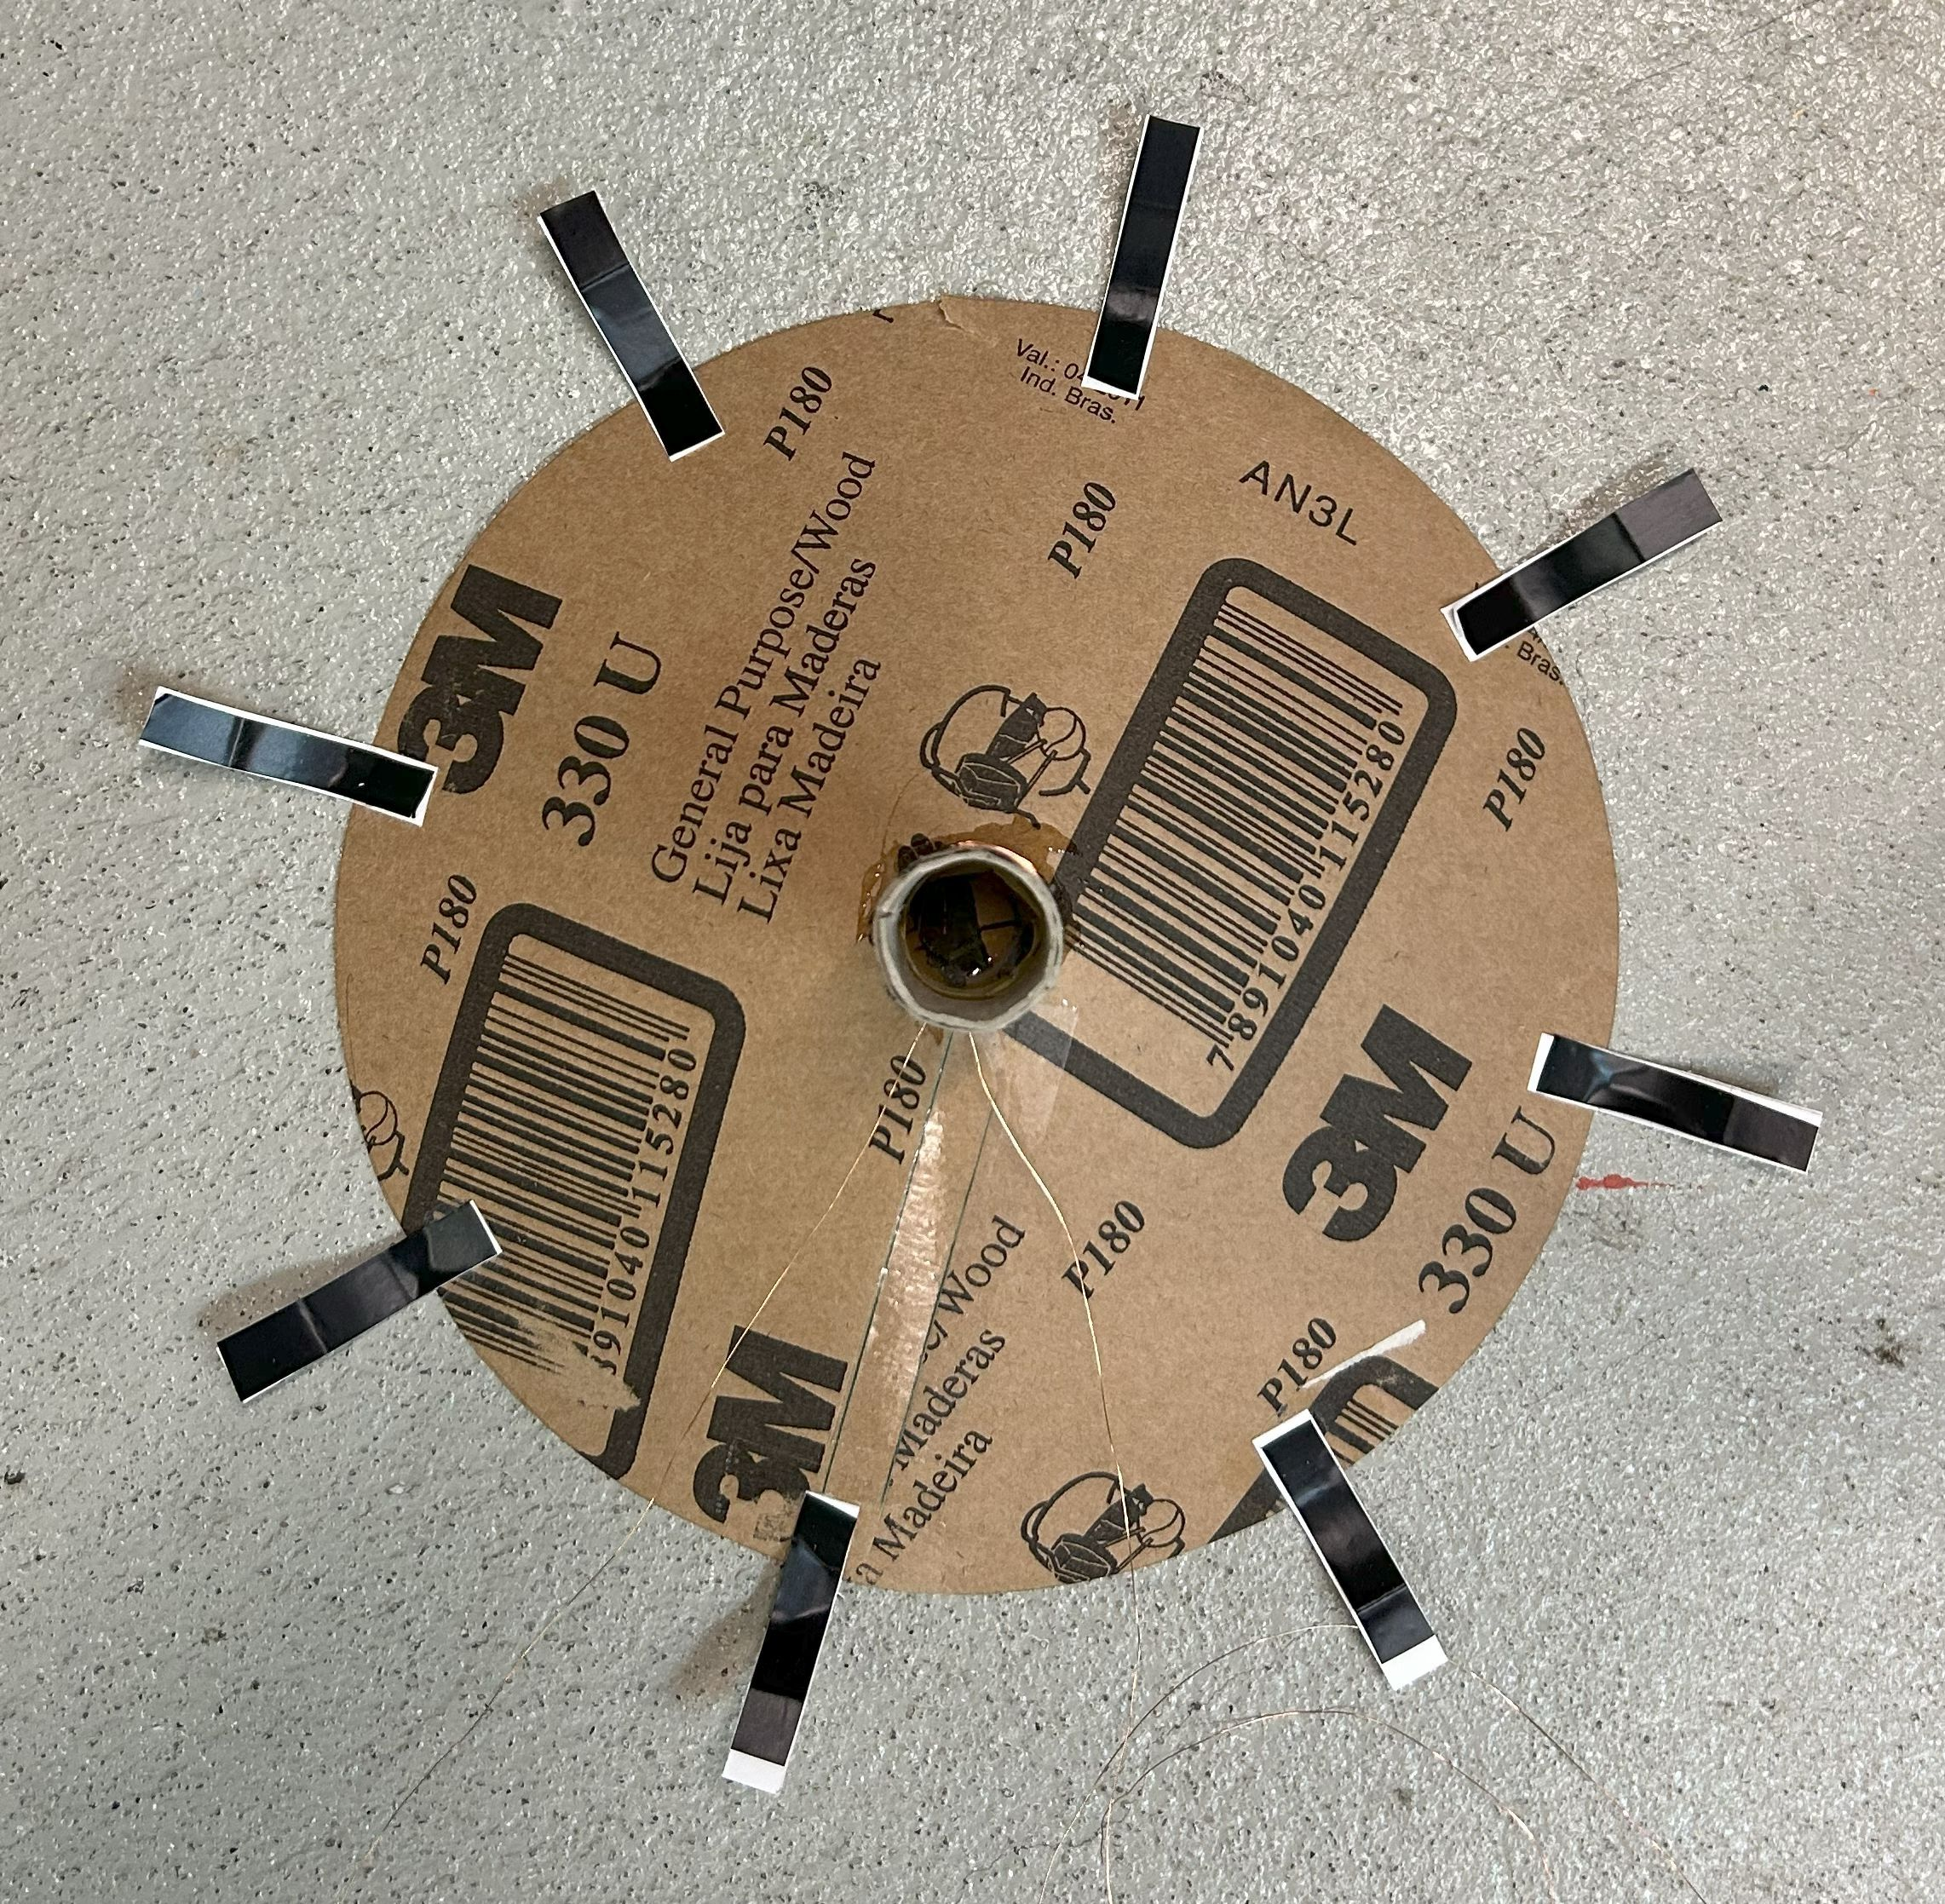
\includegraphics[width=0.5\textwidth]{resources/images/Fotos/Physik-87.jpg}
    \caption{{Fertige Membran}}
    \label{fig:membrane_fin}
\end{figure}
\newpage
\subsection{Weinkiste}
Die Wahl, eine Weinkiste als Resonanzkörper zu nehmen, wurde aufgrund deren spezifischen Eigenschaften getroffen. Holz weist ein gutes Resonanzverhalten auf und dämpft die Schwingungen, wodurch die Klänge und Frequenzen nicht verschwimmen. Die Wandstärke von 10 mm ist gross genug, damit die Wände nicht beginnen sich mit den Frequenzen zu wölben. Sie sind aber dünn genug, um mit der vom Lautsprecher verfügbaren Leistung mitzuschwingen. 

\subsection{Tieftönersicke}
Während der Entwicklung der Sicke wurden verschiedene Konzepte ausprobiert. Die W-Sicke (Typ I, siehe Abbildung 2.3) stellte sich vorerst als gute Lösung heraus. Sie besteht aus acht Sickenstreifen welche fünf Male gefaltet wurden. In Kombination mit vier Gummibändern zwischen Spule und Gestell konnte ein gutes Resultat erzielt werden. Die Gummibänder erfüllten den Zweck einer Spinne und drückten die Membran nach aussen, bis die Sickenstücke unter Spannung waren. Wenn die Membran nun zurückgezogen wurde, falteten sich die Sickenstreifen an den gewollten Stellen und die Membran konnte sich sehr frei bewegen. Diese Bewegungsfreiheit sorgte jedoch für eine sehr unklare Hochfrequenzwiedergabe. Also wurde die C-Sicke (Typ II, siehe Abbildung 2.4) entwickelt. Diese ist viel stabiler und weist lediglich zwei Faltstellen auf. Die Gummibänder erfüllen nun nur noch den Zweck der Spinne, also das exakte führen der Spule über den Magneten. Sie sind ebenfalls so in ihrer Spannung angepasst, dass die Spule (im stehenden Zustand) bei der radial wirkenden Gravitation nicht in Berührung mit dem Magneten kommt. (Siehe Abbildung 2.5) 

\begin{minipage}{0.3\textwidth}
    \centering
    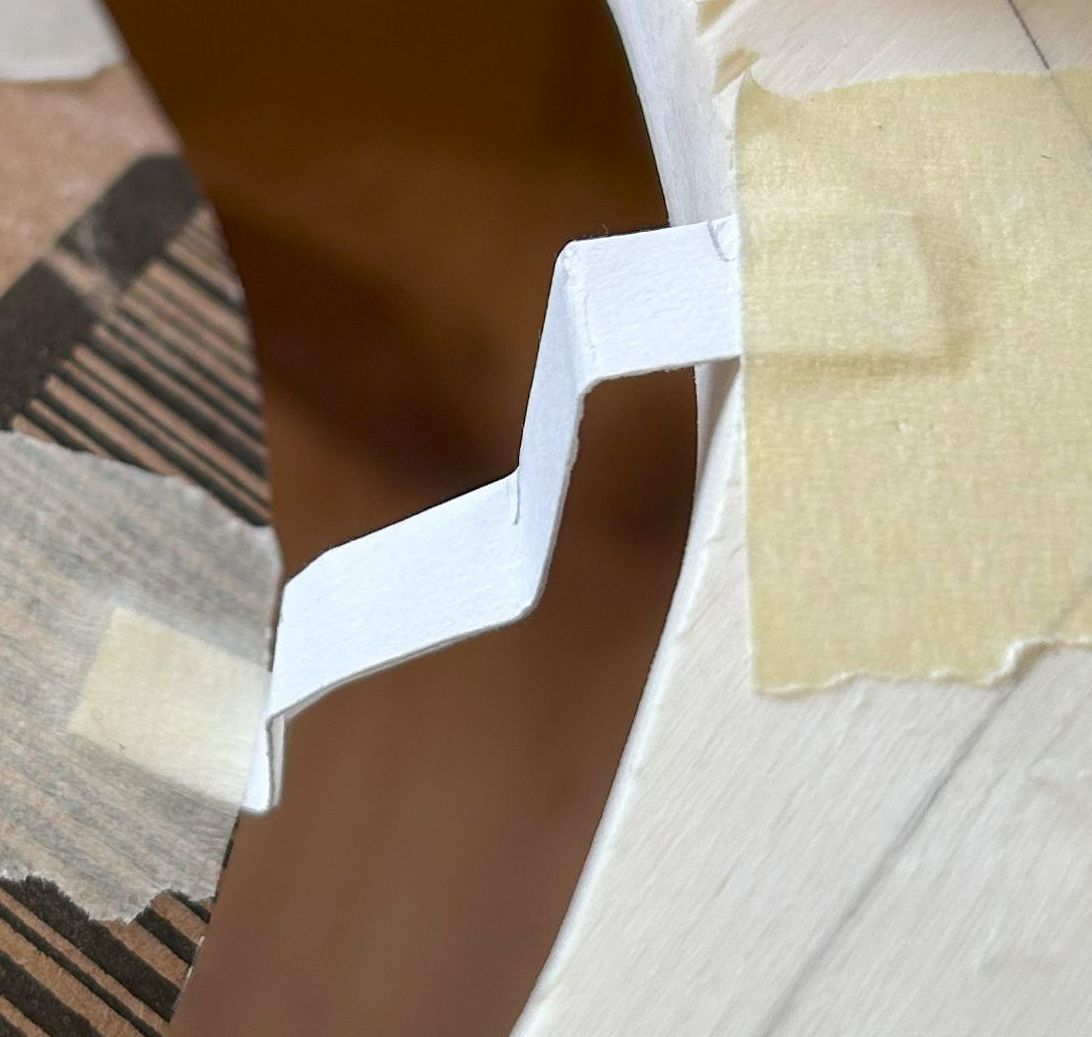
\includegraphics[width=.8\linewidth]{resources/images/Fotos/Physik-77.jpg}
    \captionof{figure}{\raggedright{W-Sickel (Typ I)}}
    \label{fig:w_sicke}
\end{minipage}
\begin{minipage}{0.3\textwidth}
    \centering
    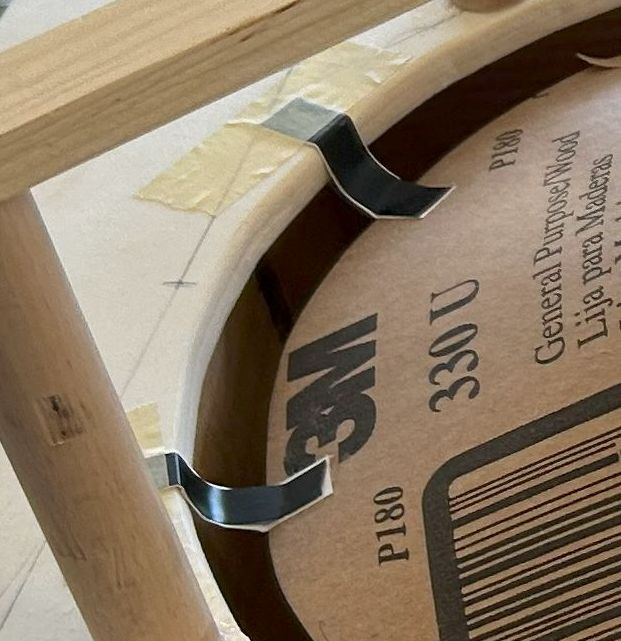
\includegraphics[width=.8\linewidth]{resources/images/Fotos/Physik-96.jpg}
    \captionof{figure}{\raggedright{C-Sicke (Typ II)}}
    \label{fig:c_sicke}
\end{minipage}
\begin{minipage}{0.3\textwidth}
    \centering
    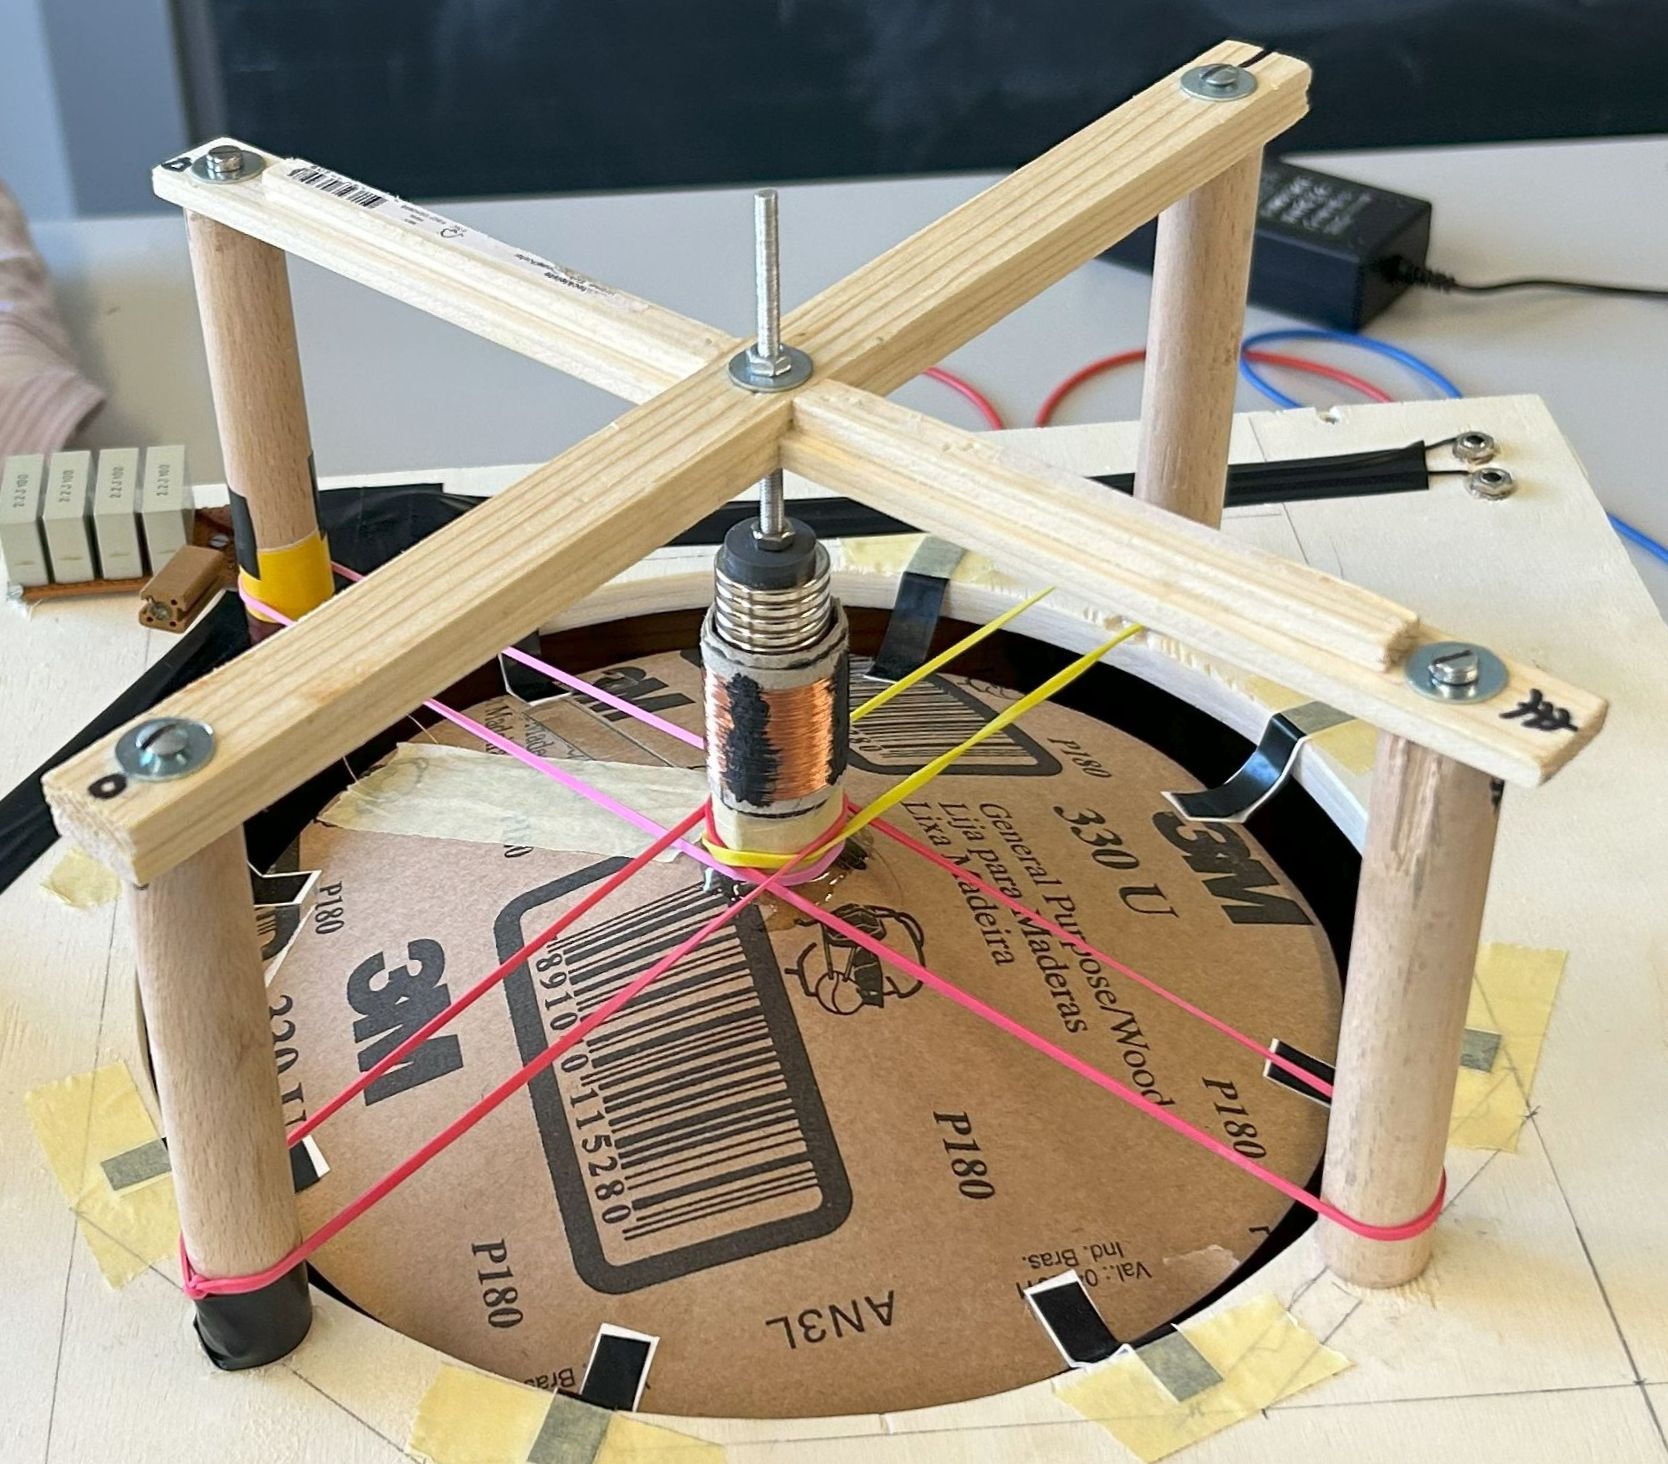
\includegraphics[width=.8\linewidth]{resources/images/Fotos/Physik-119.jpg}
    \captionof{figure}{\raggedright{Fertiger Tieftöner}}
    \label{fig:deep_fin}
\end{minipage}

\newpage
\subsection{Hochtöner}
Der Hochtöner wurde erst nachträglich installiert, da sich herausstellte, dass die Tieftönermembran trotz der neuen C-Sicke zu viel Bewegungsfreiraum hat, um hohe Frequenzen, welche vorallem in Stimmen sehr wichtig sind, klar wiederzugeben. Aus diesem Grund wurde ein zweiter Lautsprecher mit viel kleinerer Membran, ein Hochtöner, gebaut. Dieser weist über eine sehr steife Sicke auf, welche aus Strohhalmen konstruiert wurde. Dies ermöglicht die Wiedergabe von Frequenzen von über 15'000Hz. Der Platz, welcher der Hochtöner einnimmt war ursprünglich für ein Bassreflexrohr angedacht. Die Hochtönerspule hat 200 Wicklungen und weist eine Impedanz von 7,7\Omega\  auf. Er wurde als eigenständiges Modul konstruiert und dann eingebaut.

\subsection{Bassreflexrohr}
Zu beginn war die Idee, ein Bassreflexrohr in den Lautsprecher einzubauen. Ein solches sollte die Qualität der Basswiedergabe verbessern. Dafür wäre es nötig, dass das Gehäuse bis auf das Loch für das Rohr komplett luftdicht verschlossen sein muss. Dies war mit der Weinkiste nicht zu erreichen. Entsprechend wurde dann entschieden, dass ein zusätzlicher Hochtöner gebaut werden sollte, welcher dann den Platz und das Loch für das Bassreflexrohr eingenommen hat. Trotzdem wurde versucht, die Kiste so gut wie nur möglich mit Holzfaser- und Reparaturspachtel abzudichten. 

\subsection{Magnet-Stelleinheit}
Um die Neodymmagneten des Tieftöners auf eine möglichst effiziente Funktionsweise justieren zu können, wurde ein System entwickelt, welches aus den Magneten und einer Gewindstange besteht. Dabei kann die gesamte Gewindestange inklusive Magneten näher zur Membran oder weg davon bewegt und an der entsprechende Stelle fixiert werden. Dabei wurden selbstverständlich nur nicht ferromatgnetische Materialien verwendet, damit das Magnetfeld nicht beeinflusst wird. Die fertige Magnet-Stelleinheit ist auf der Abbildung 2.6 zu sehen. 

\begin{figure}[h]
    \centering
    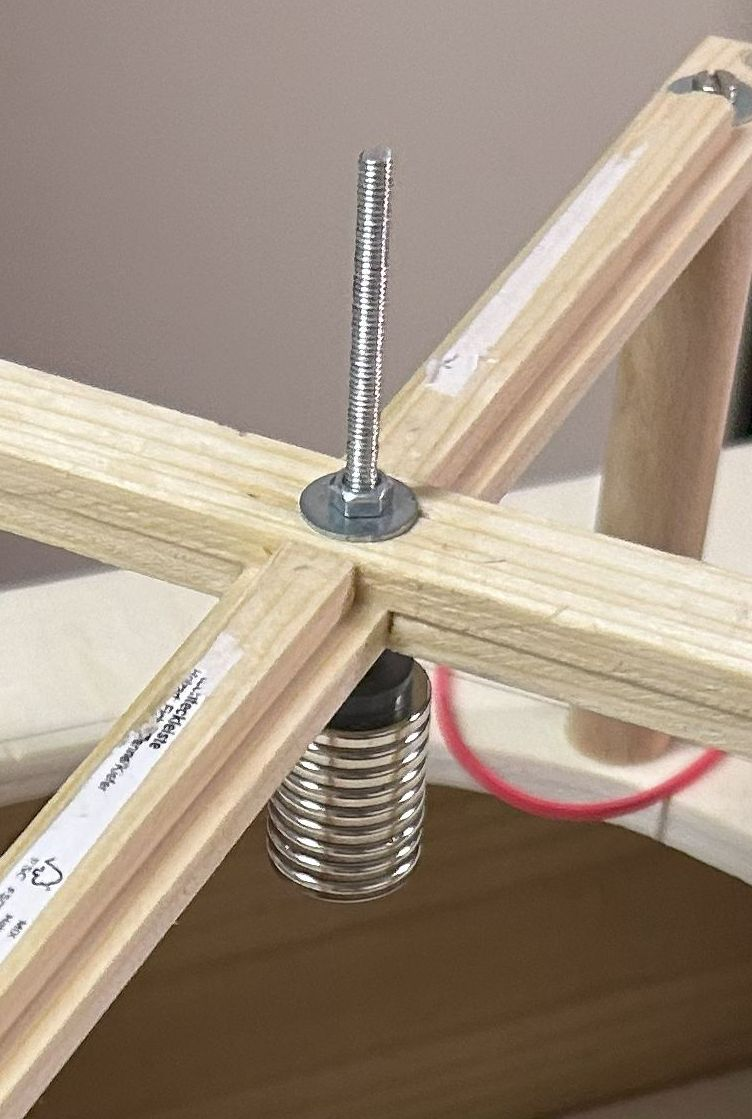
\includegraphics[width=.3\linewidth]{resources/images/Fotos/Physik-86.jpg}
    \caption{{Magnet-Stelleinheit}}
    \label{fig:magnet}
\end{figure}

\newpage
\subsection{Elektrik}
\subsubsection*{Hitze}
Hauptverantwortlich für die Hitzeentwicklung sind die tiefen Frequenzen. Sie weisen den grössten Membranhub auf und brauchen auch die meiste Energie. Aufgrund der Grösse der Tieftönerspule konnte diese die Wärme stehts gut abführen. Viel eher lag das Problem in der Ungleichverteilung der Stromstärke aufgrund der beiden unterschiedlichen Widerstände. So war die Stromstärke des Hochtöners mit 7,7\Omega\ viel grösser als die des Tieftöners. Somit wurde dieser schnell heiss, und die Höhen wurden zu laut wiedergegeben. Also wurde ein 7,2\Omega\ Widerstand in den Stromkreis integriert. Somit wird viel eher der Wiederstand als die Spule heiss und die Frequenzen sind in ihrer Lautstärke ausgeglichen. Zusätzlich wurde die Spule absichtlich nicht mit Ofenschnurkleber eingedeckt um keine Isolationsschicht zu schaffen und eine bessere Luftkühlung zu ermöglichen.
\subsubsection*{Frquenzselektion und Filterung}
Da bemerkt wurde, dass der Hochtöner beim Versuch tiefe Frequenzen wiederzugeben, stark zu klappern begann sollte zuerst eine Frequenzweiche gebaut werden. Diese benötigt jedoch genau aufeinander abgestimmte Bauteile. Diese waren so nicht verfügbar. Speziell die Kondensatoren welche über eine ausserordentlich hohe Kapazität von 40\mu F aufweisen müssten. Zwar wurde eine Frequenzweiche mit nicht perfekt abgestimmten Bauteilen gebaut (siehe Abbildung 2.7), welche die Tonqualität auch verbesserte, jedoch wurden versehentlich Elektrolytkondensatoren verwendet. Diese gehen bei Wechselspannung kaputt und sind somit nicht für diese Anwendung geeignet. 

Da die Frequenzweiche selbst mit den passenden Teilen vermutlich nicht äusserst präzise funktioniert hätte, sollte nun lediglich ein Hochpassfilter, welcher die tiefen Frequenen entfernt, auf den Hochtöner angewendet werden. Dieser Filter (siehe Abbildung 2.8) wurde aus vier 2,2\mu F Folienkondensatoren gebaut und in den Lautsprecher integriert. Dies führte (bei 8,8\mu F) zu einer Eckfrequenz von 150Hz welche für die Lautsprecher optimal ist. 

\begin{minipage}{0.5\textwidth}
    \centering
    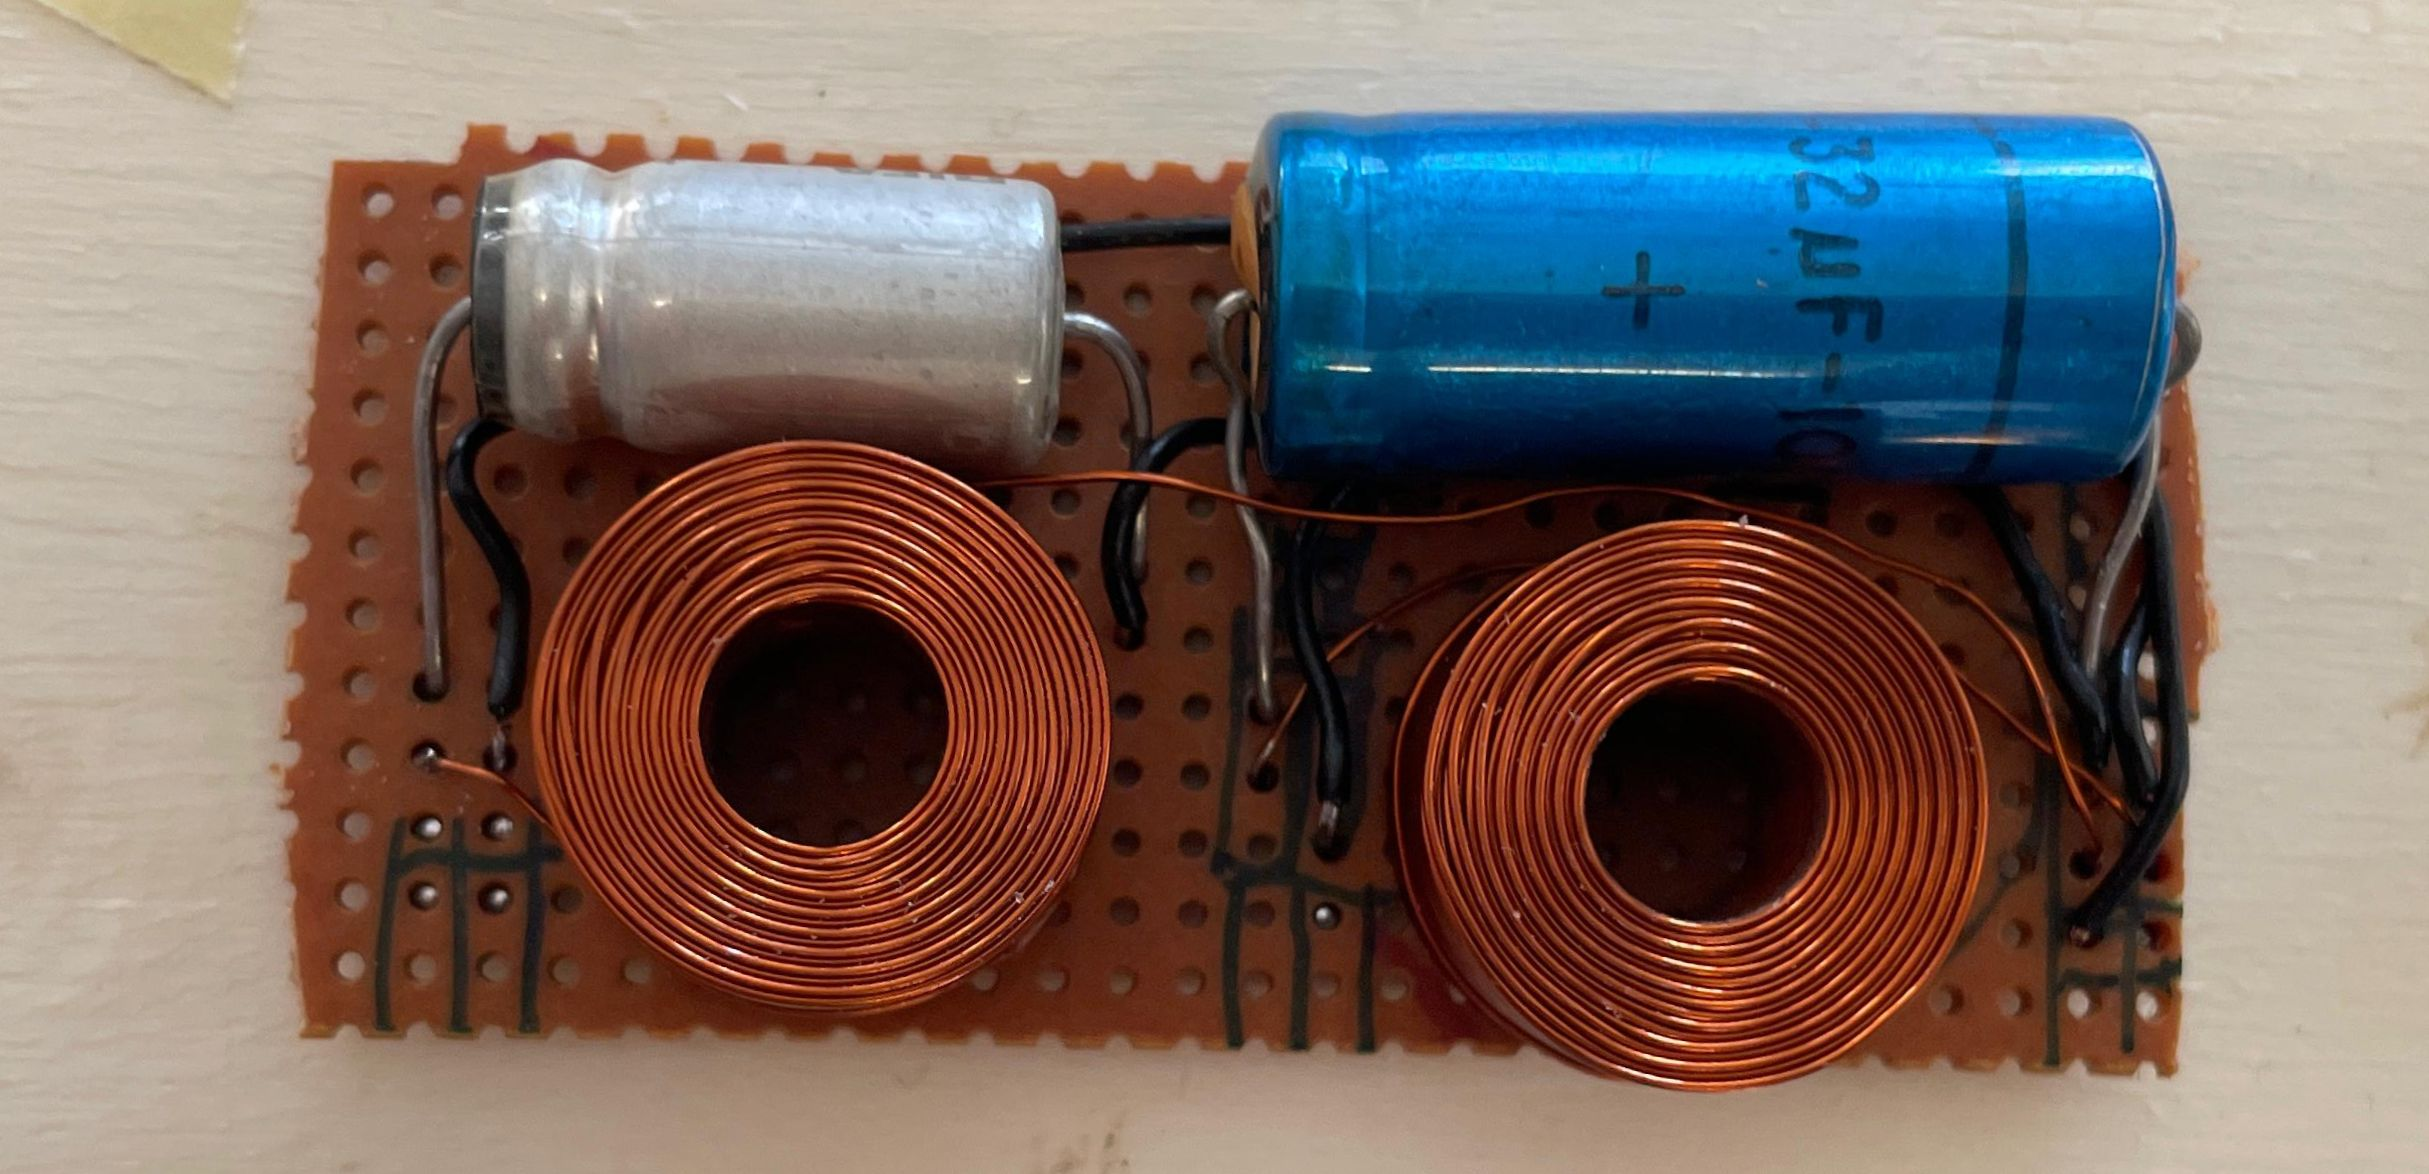
\includegraphics[width=.8\linewidth]{resources/images/Fotos/Physik-138.jpg}
    \captionof{figure}{\raggedright{Frequenzweiche}}
    \label{fig:weiche}
\end{minipage}
\begin{minipage}{0.5\textwidth}
    \centering
    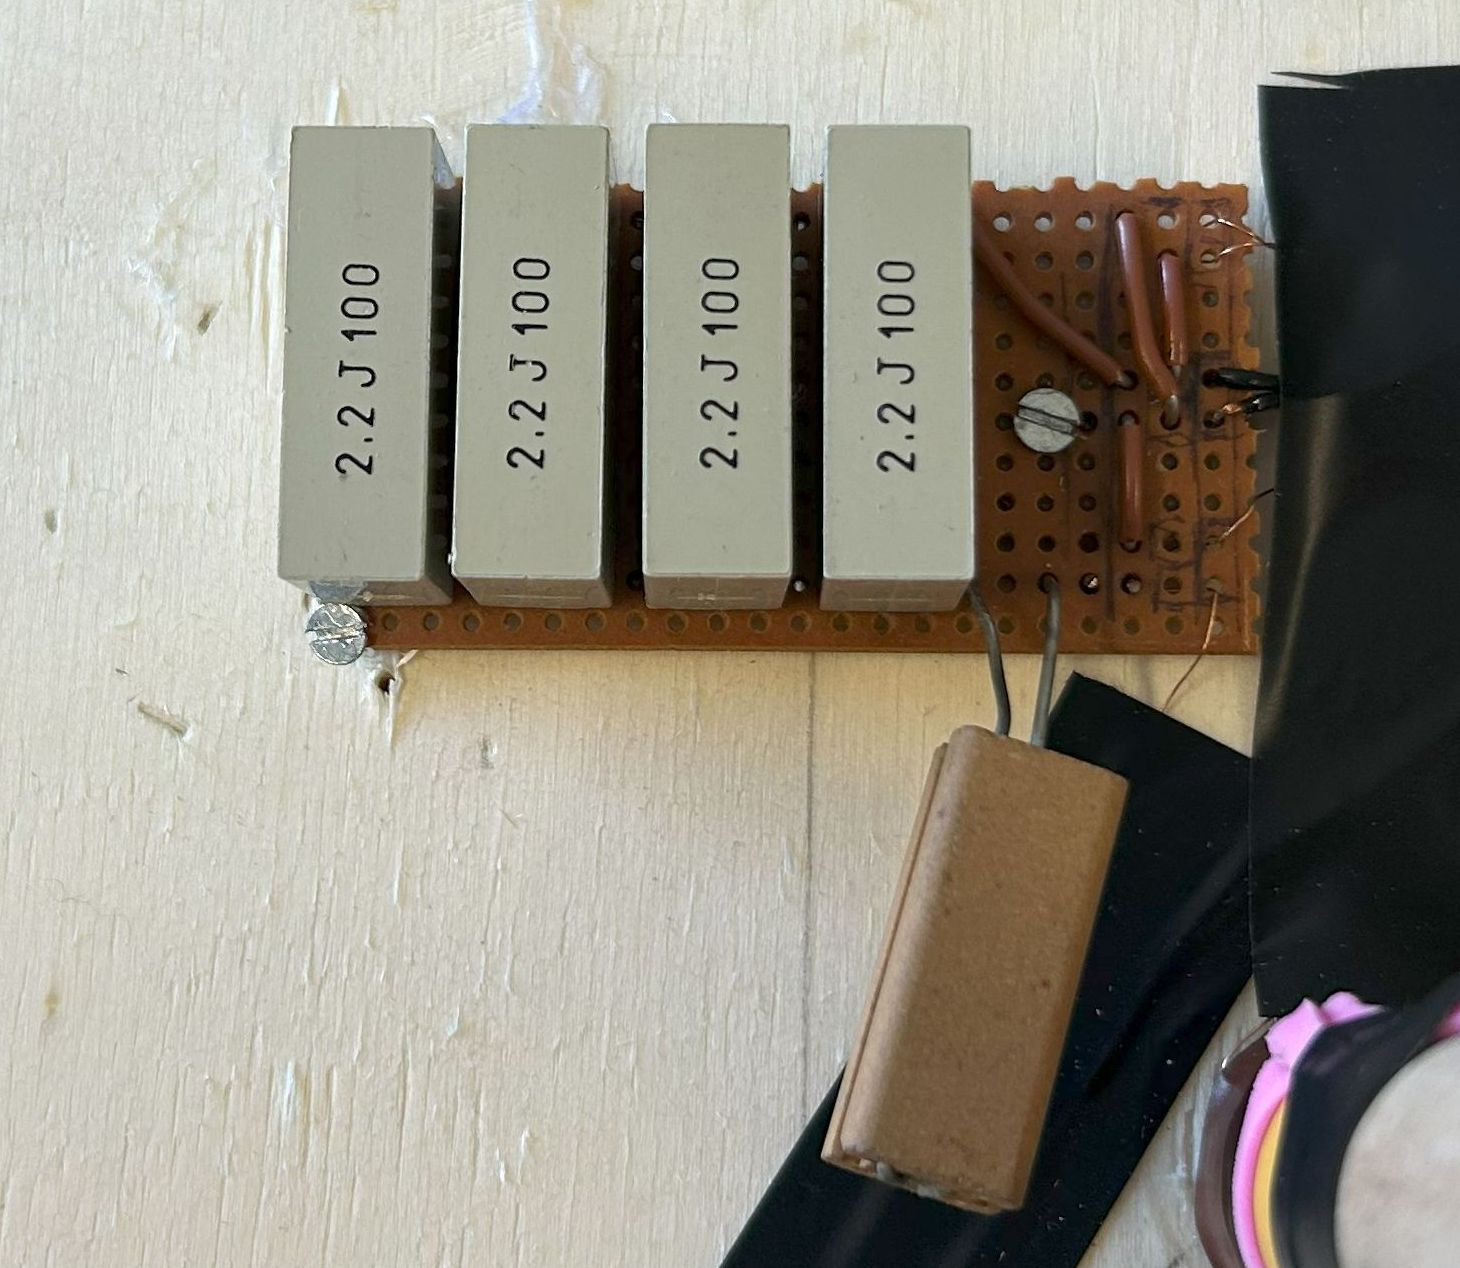
\includegraphics[width=.8\linewidth]{resources/images/Fotos/Physik-127.jpg}
    \captionof{figure}{\raggedright{Hochbassfilter}}
    \label{fig:filter}
\end{minipage}

\newpage
\section{Methoden}
Es wurde viel im Internet recherchiert, um herauszufinden wie bestimmte Bauteile optimal konstruiert werden können. Zudem versuchte man auch durch Versuche optimale Ausführungen mit den zur Verfügung stehenden Materialien zu finden.

Sehr viel wurde im Physiklabor mit grosser Unterstützung des Laboranten erarbeitet. Zudem wurde zu Hause auch laufend weitergebaut. Der grösste Aufwand des ganzen war das handwerkliche Bauen des Lautsprechers selbst.

Ebenfalls wurden CAD Programme verwendet, um einen Plan des gesamten Lautsprechers zu erstellen.

\chapter{Resultate}

\section{Ergebnisse Tieftöner}
Der Tieftöner wurde als erste Etappe des Lautsprechers gebaut. Der Klang des Tieftöners ist für einen aus Haushaltsmaterialien selbstgebauten Lautsprecher hervorragend. Allerdings hat der Tieftöner allein Probleme, hohe Frequenzen wahrheitsgetreu wiederzugeben. Beispielsweise sind die Stimmen in Filmen sehr undeutlich und somit schlecht zu verstehen. Die Basswiedergabe ist jedoch sehr zufriedenstellend.

\section{Ergebnisse Hochtöner}
Da die Gruppe der Meinung war, dass der Tieftöner allein nicht ausreicht, wurde ein Hochtöner gebaut. Der Hochtöner erfüllt seinen Zweck hervorragend und lässt vorallem Stimmen klar und deutlich erscheinen. Die tiefen Töne, welche für die klappernden Klänge verantwortlich waren, konnten mit dem Akustikfilter vollständig eliminiert werden. Bei gewissen Frequenzen gerät der Hochtöner in Eigenresonanzbewegungen. Der Klang wird dann leicht metallig und klirrend, jedoch erklingen die Frequenzen stets sehr akurat. Dies könnte mit einem Wechsel von reinen Sinus- auf Rechteckwellen verglichen werden. Durch den zusätzlichen Widerstand sind die Lautstärken der beiden Lautsprecher nun optimal ausgeglichen.

\section{System mit Akustikfilter}
Der eingebaute Hochpassfilter verbessert den Klang um ein Vielfaches. Der Filter erwies sich als die und am bestmöglich umsetzbare Lösung.
\chapter{Reflexion}

In einem Zeitraum von zwei Monaten gelang es, das Ziel, einen selbstgebauten Lautsprecher zu konstruieren, vollständig zu erreichen. Die schliesslich erreichte Tonqualität ist als gut zu bezeichnen, was durch die Kombination eines Hochtöners mit einem Tieftöner erreicht werden konnte. Darüber hinaus konnte die Gruppe ihr Wissen im Bereich der Elektrik und Akustik erweitern. 

\section{Bauprozess}
Der Bauprozess wurde in verschiedene Phasen unterteilt, in denen kontinuierlich nach potenziellen Optimierungen gesucht wurde, die schlussendlich zum Endresultat führten.

In der ersten Phase wurde eine Form eines Lautsprechers mit einer einzelnen, grossen Membran (in den folgenden Phasen der Tieftöner) gebaut und in eine Weinkiste integriert. In einem Zeitraum von wenigen Wochen gelang es der Gruppe, diesen Lautsprecher zu konstruieren. Das erzielte Ergebnis wurde jedoch als zu basslastig empfunden. Positiv anzumerken ist jedoch, dass in dieser Phase Wissen und Ideen für Optimierungen gewonnen werden konnten. In der darauffolgenden Phase wurde daher die Entscheidung getroffen, einen Hochtöner zu installieren, der parallel zum Tieftöner geschaltet wird. 

Die Fertigung und Installation des Hochtöners konnte innerhalb weniger Tage erfolgreich abgeschlossen werden. Der verringerte Zeitaufwand kann auf die gewonnenen Erfahrungen zurückgeführt werden. Anfänglich wurden die Lautsprecher ohne weitere Bauteile parallel an den Verstärker angeschlossen. Die Integration des Widerstandes resultierte in einer signifikant positiven Beeinflussung der Tonqualität. Nichtsdestotrotz wurde ein zusätzliches Optimierungspotenzial identifiziert, welches durch die Implementierung eines Akustikfilters erschlossen werden sollte, um eine weitere Steigerung der Tonqualität zu erreichen.

Der Bau der nicht verwendeten Frequenzweiche und des funktionierenden Filters erforderte einen erheblichen Zeitaufwand. Das Hauptproblem bestand darin, dass die erforderlichen Kondensatoren nicht zur Verfügung standen, sodass keine funktionierende und sichere Frequenzweiche konstruiert werden konnte. In der Folge wurde der Entschluss gefasst, den entsprechenden Hochpassfilter zu konstruieren.

In der finalen Bauphase wurde dieser Filter konstruiert. Der Bauprozess gestaltete sich jedoch als komplex und zeitintensiv, was zu gewissen Herausforderungen führte.        

\newpage
\section{Technische Erkenntnisse}
Im Hinblick auf die Spule des Tieftöners wurde die Anzahl der Wicklungen eines 0,2mm dicken Kupferdrahtes auf 400 festgelegt. Diese Entscheidung resultierte aus einer Reihe von Versuchen mit unterschiedlichen Spulen mit unterschiedlichen Wicklungen. Das Resultat dieser Bemühungen zeigt sich in einer optimalen Frequenzwiedergabe im Tieftonbereich, die insbesondere durch das gute Prototyping ermöglicht wurde.

Ein weiterer entscheidender Faktor war die Notwendigkeit, eine Überhitzung der Spule zu verhindern. Aus diesem Grund wurde ein Drahtdurchmesser von 0,2mm für die Spule als optimal erachtet. Die Membran wurde aus Schleifpapier gefertigt, da sich dieses Material als robust erwies und sich als vorteilhaft herausstellte. 

In Bezug auf den Hochtöner wurde der selbe Drahtdurchmesser verwendet, da dieser bereits erprobt und als geeignet befunden wurde. Bei den Wicklungen wurde eine Anzahl von 200 gewählt, da die Membran deutlich weniger stark schwingen sollte als beim Hochtöner. Die Temperatur stellt beim Hochtöner mit entsprechendem Widerstand kein Problem mehr dar, da deutlich weniger Strom durch die Spule fliesst. Ebenso wurde bei dieser Membran auf Schleifpapier gesetzt, da beim Tieftöner gute Resultate erzielt werden konnten.

Die vorliegende Untersuchung kommt zu dem Schluss, dass die Klangqualität des Lautsprechers durch die abgedichtete Weinkiste positiv beeinflusst wird. Aus diesem Grund wurden bis auf die Abdichtung keine weiteren Änderungen an der Kiste selbst vorgenommen.

Die korrekte Verkabelung im Inneren des Lautsprechers war ein sehr wichtiger Schritt, um das Vibrieren der Kabel während des Betriebs des Lautsprechers zu vermeiden. Zu diesem Zweck wurden die Kabel und Drähte mittels Isolierband direkt an das Holzkonstrukt geklebt.

Das Gestell, in welchem sich die Spule, der Magnet und die Membran befinden, muss eine hohe Robustheit aufweisen. Aus diesem Grund wurde für den Tieftöner eines aus Holz konstruiert, während für den Hochtöner ein stabiles Kartonkonstrukt gebaut wurde.

\section{Kritische Reflexion des Prozesses}
Der Bauprozess verlief im Allgemeinen zufriedenstellend. Allerdings wäre eine Optimierung des Zeitmanagements noch als möglich zu erachten gewesen. So wurde beispielsweise für den Bau der Frequenzweiche ein erheblicher Zeitraum aufgewendet, der sich am Ende als unnötig herausstellte, da man die falschen Kondensatoren verwendete. Hätte man sich im Vorfeld mit den Eigenschaften der Kondensatoren auseinandergesetzt, hätte man gemerkt dass der Bau einer Frequenzweiche mit den vorhandenen Teilen nicht möglich ist.

\newpage
\section{Ergebnis}
Das Endprodukt ist als zufriedenstellend zu bewerten. Die Soundqualität des Lautsprechers ist für einen eigenhändig konstruierten Lautsprecher auf gymnasialem Niveau als eher überdurchschnittlich zu bewerten. Es wurde jedoch ein leises Klappern und Vibrieren festgestellt, das je nach Tonfrequenz und Lautstärke variiert und von Eigenresonanzbewegungen verursacht wird. Die Behebung dieses Problems erweist sich als äußerst herausfordernd, weshalb keine Maßnahmen zur Verbesserung der Membran ergriffen wurden. Erfreulicherweise ist das klappern jedoch kaum wahrnehmbar, sofern nicht speziell darauf geachtet wird. Wie das Endprodukt aussieht ist auf den Abbildungen 4.1 \& 4.2 zu erkennen.

\begin{minipage}{0.5\textwidth}
    \centering
    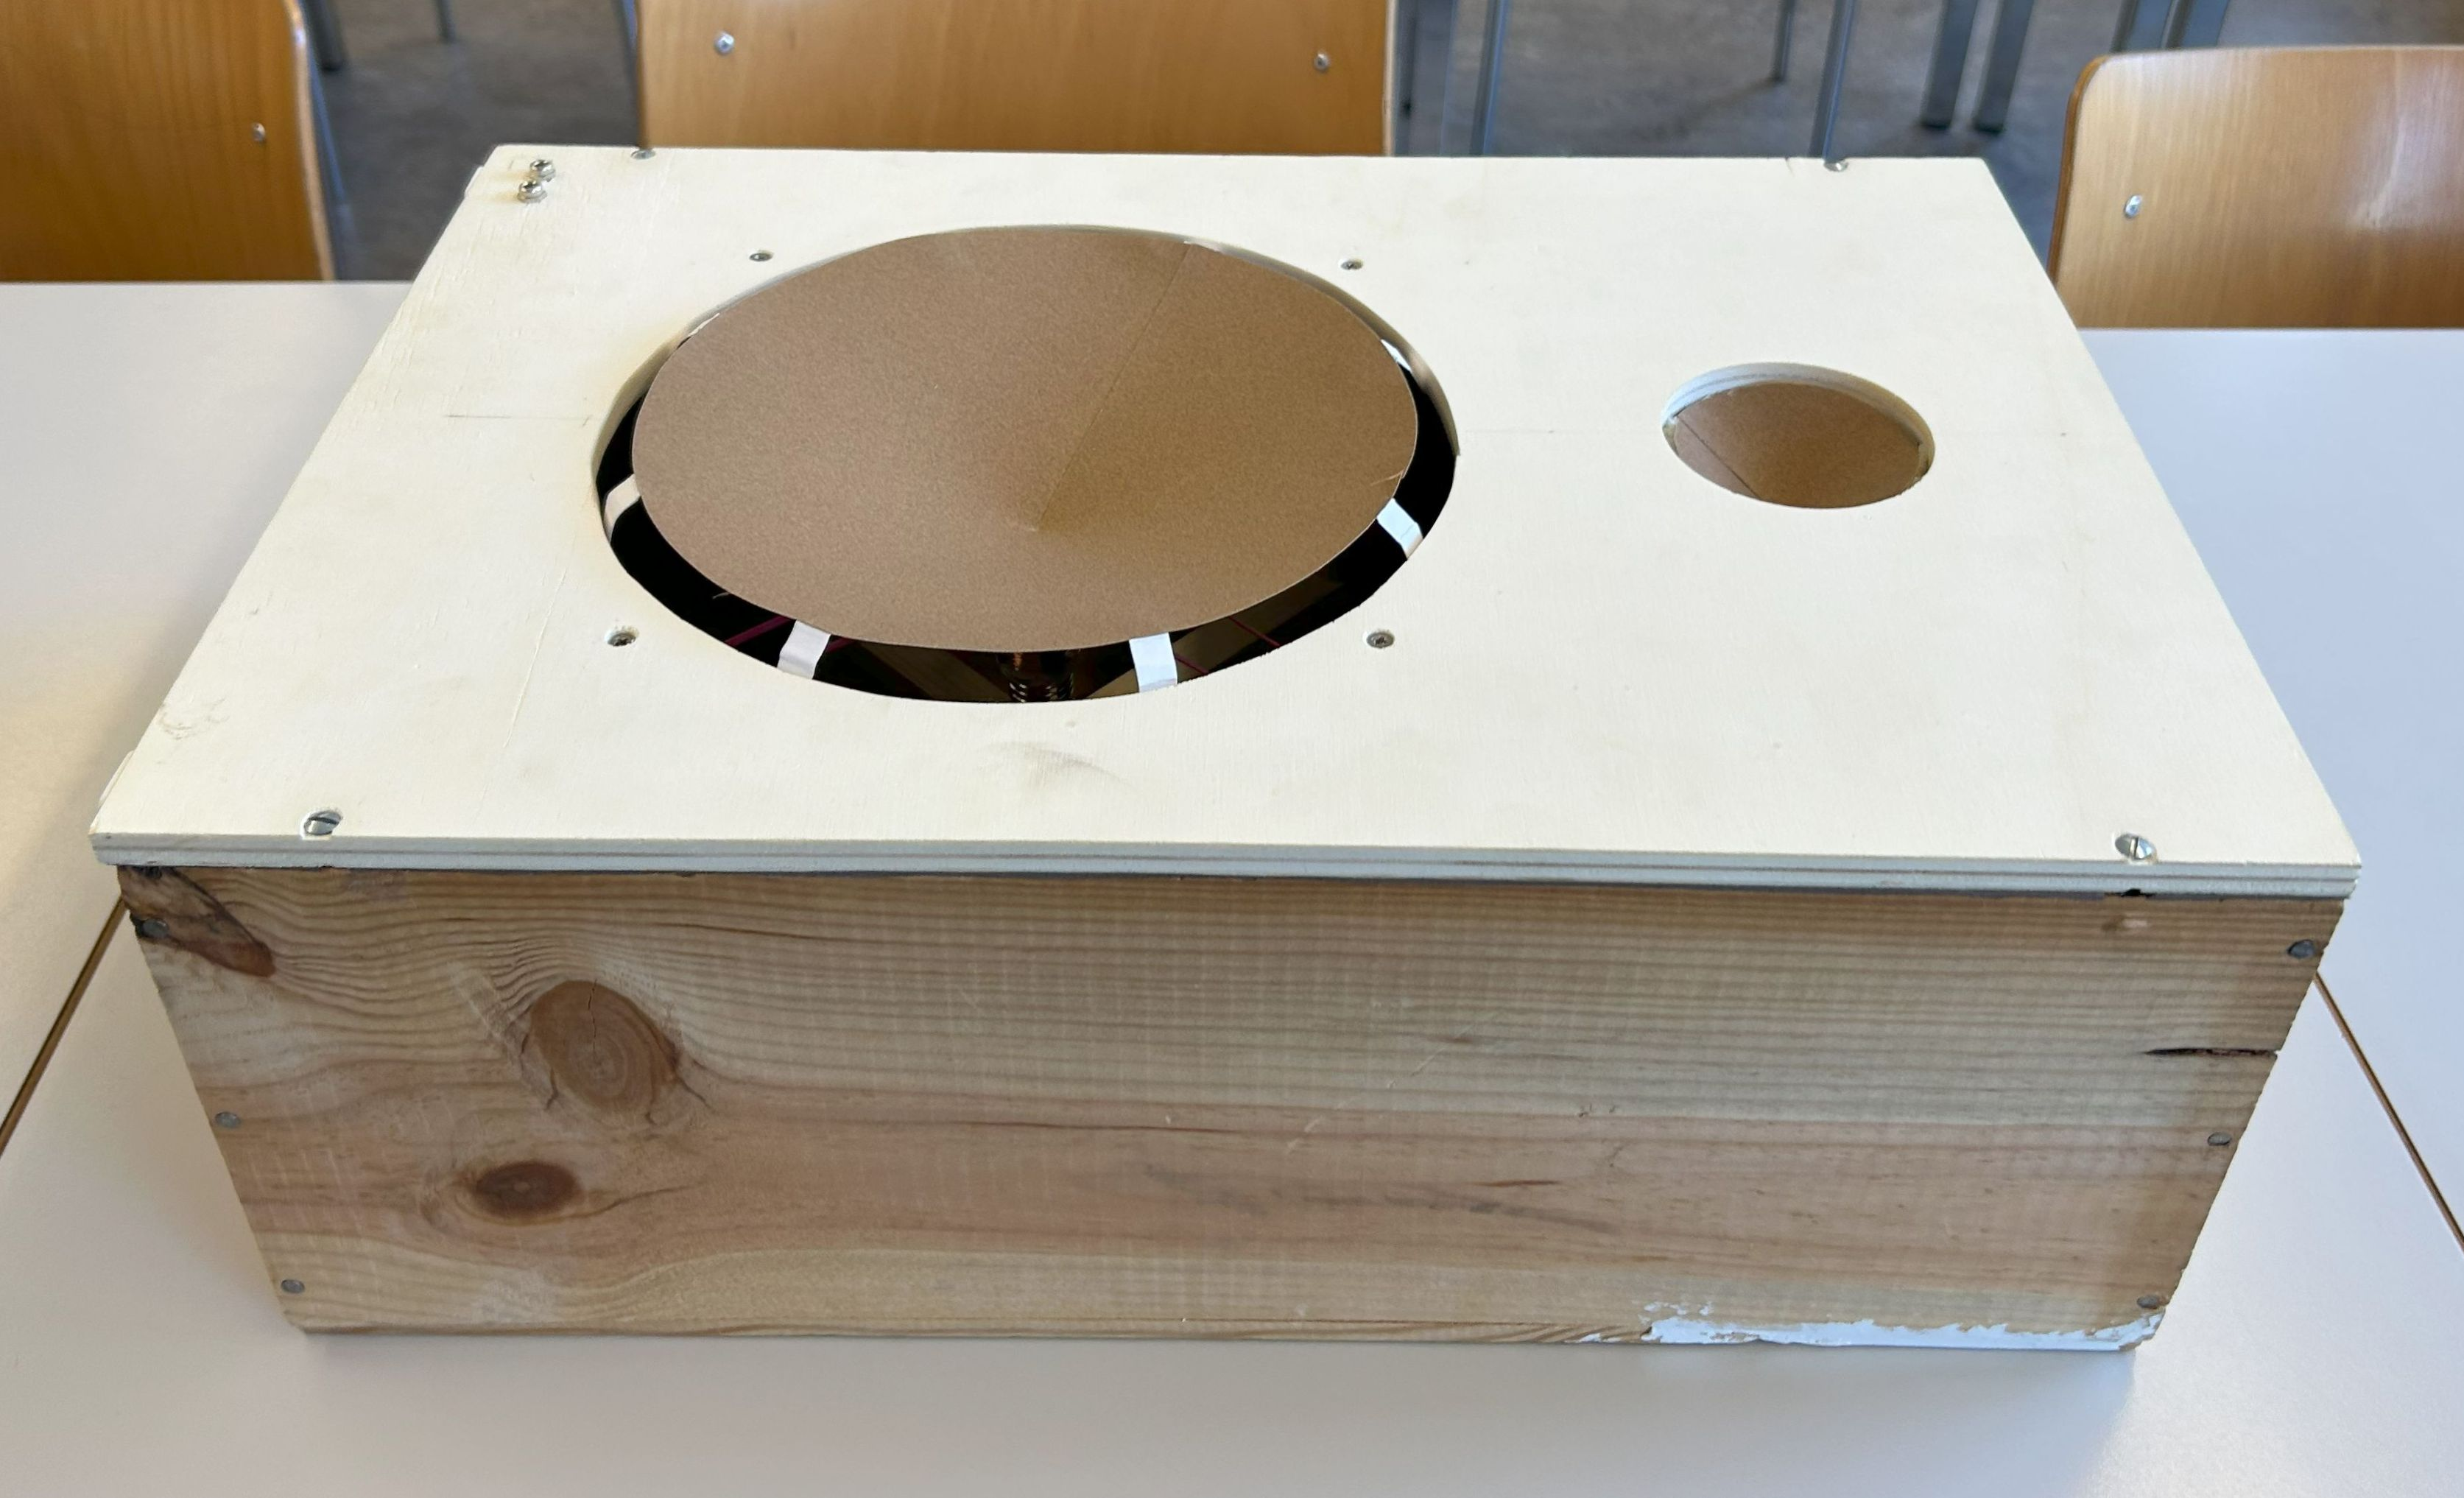
\includegraphics[width=.8\linewidth]{resources/images/Fotos/Physik-131.jpg}
    \captionof{figure}{{Lautsprecherbox von oben}}
    \label{fig:total}
\end{minipage}
\begin{minipage}{0.5\textwidth}
    \centering
    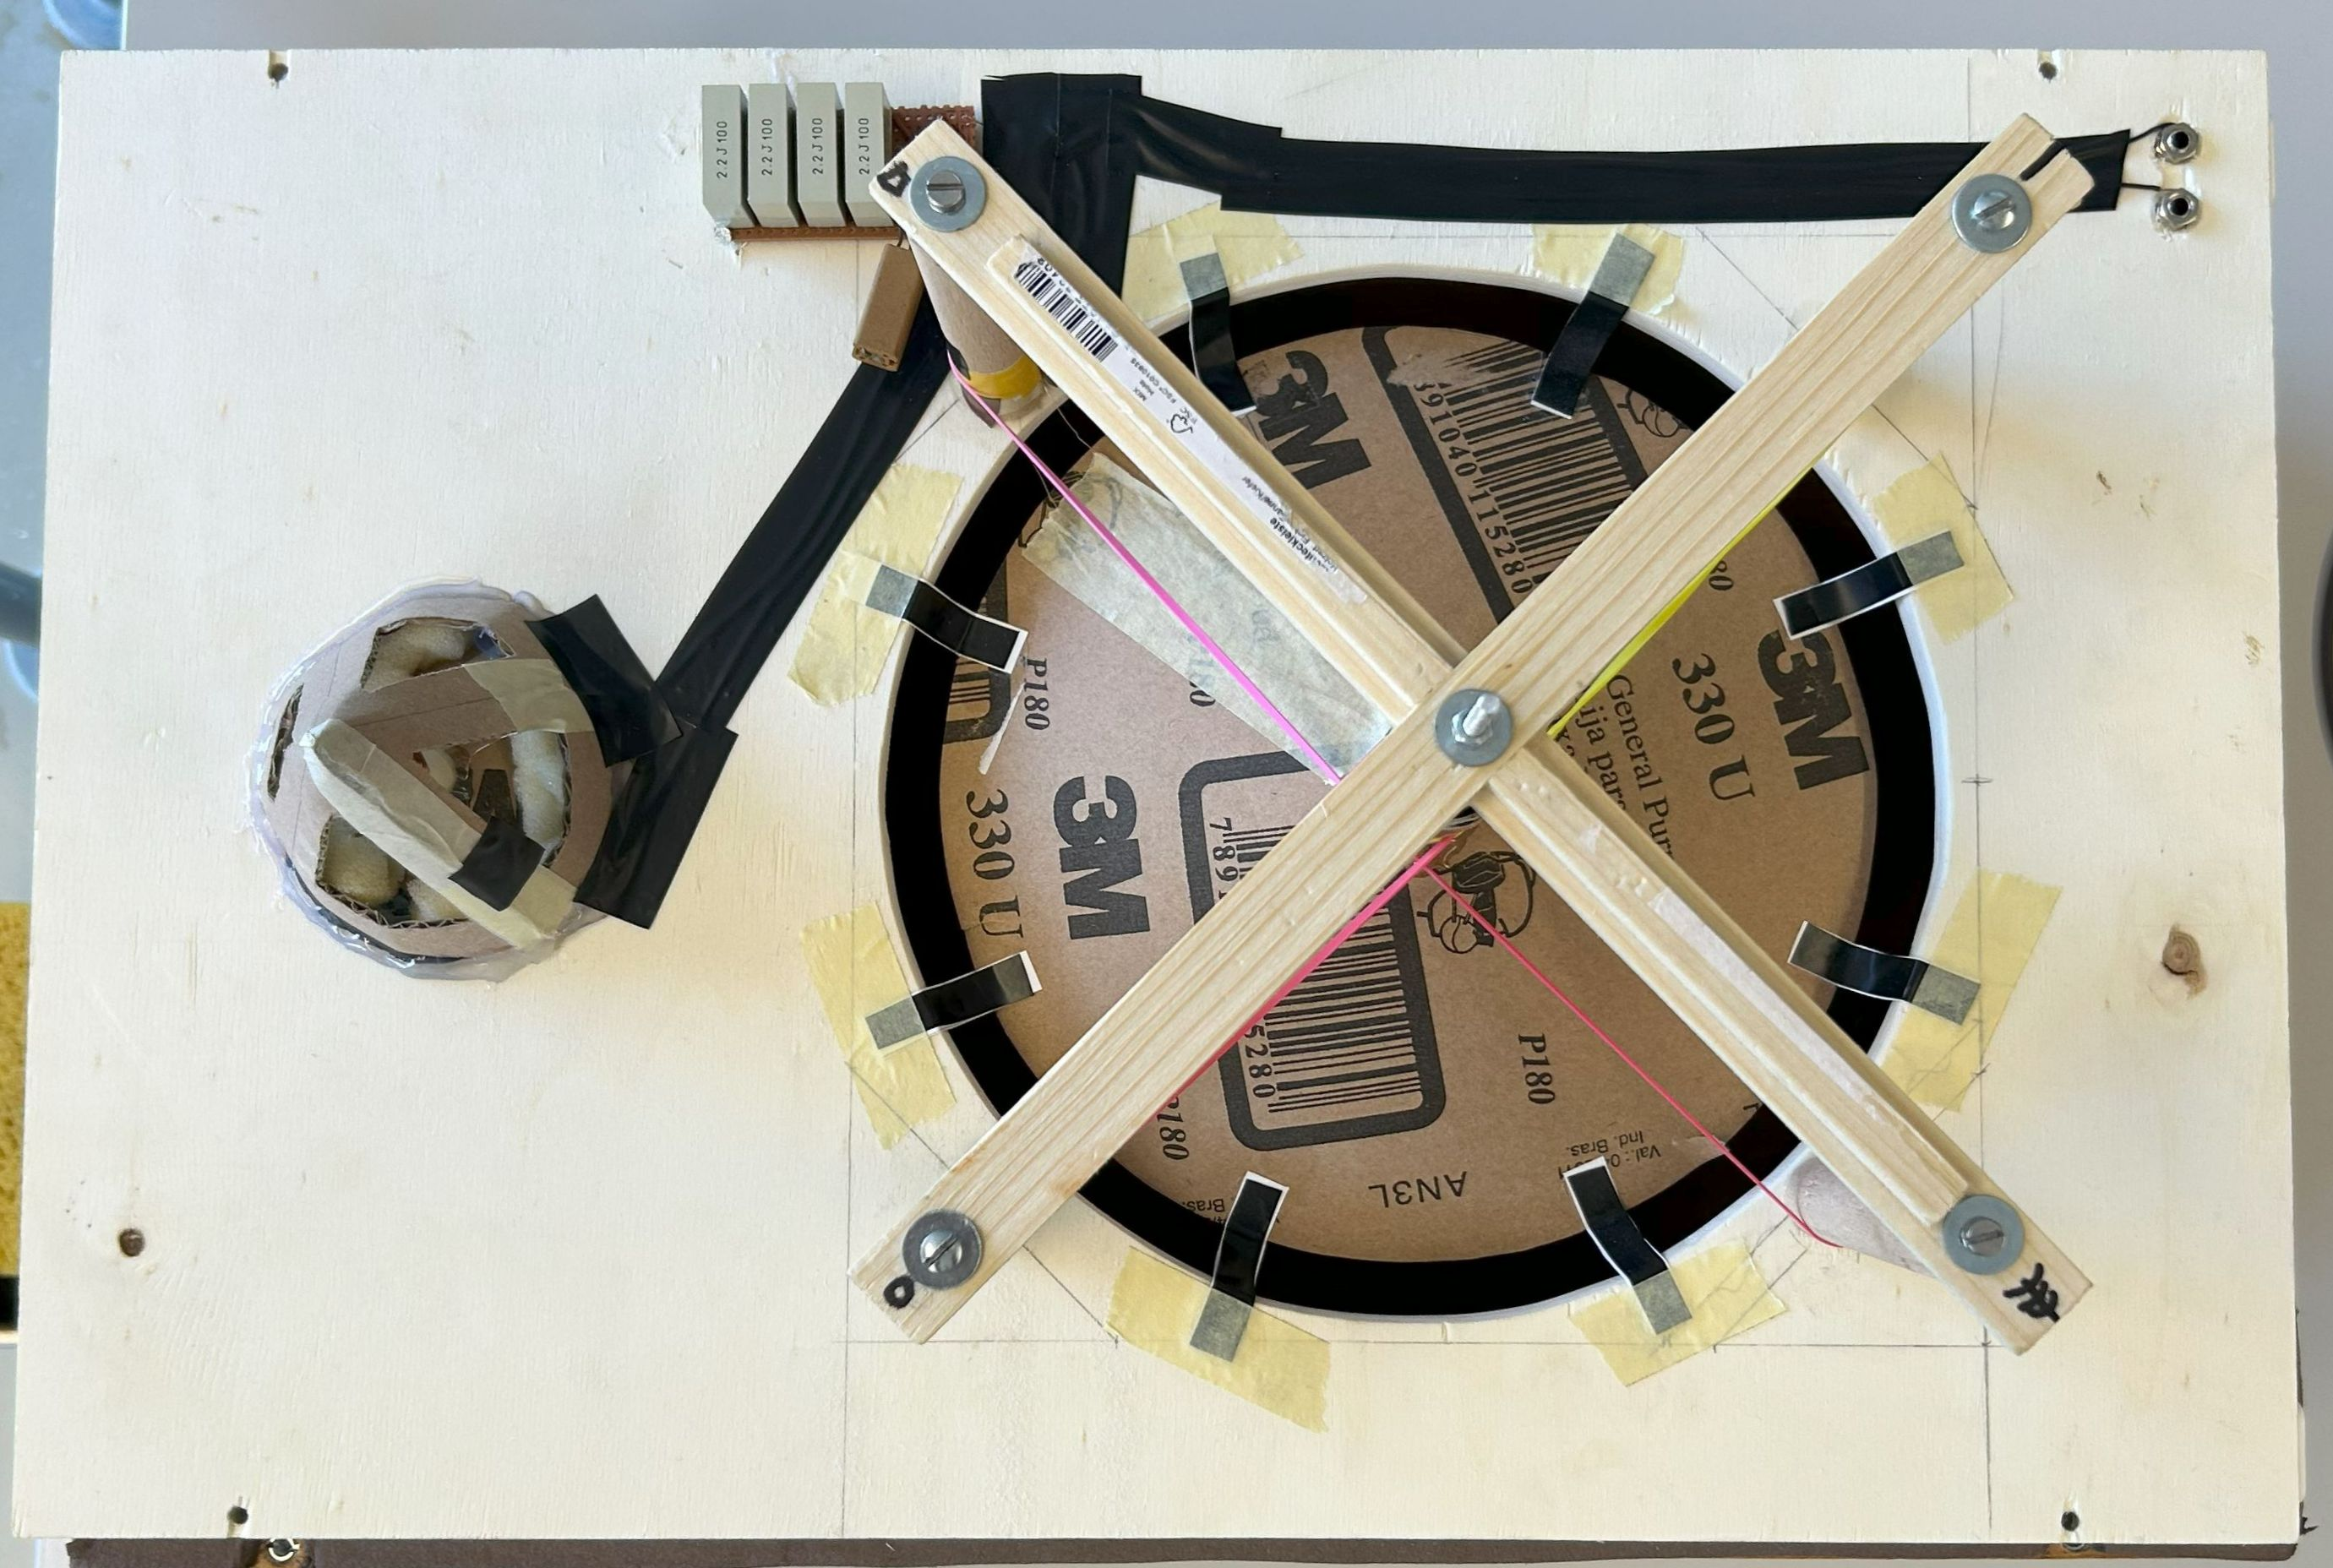
\includegraphics[width=.8\linewidth]{resources/images/Fotos/Physik-121.jpg}
    \captionof{figure}{{Deckplatte von innen}}
    \label{fig:plate_top}
\end{minipage}
% Baudokumentation
\part{Baudokumentation}

% How to build it
\chapter{Plan}
\section{CAD Zeichnung}
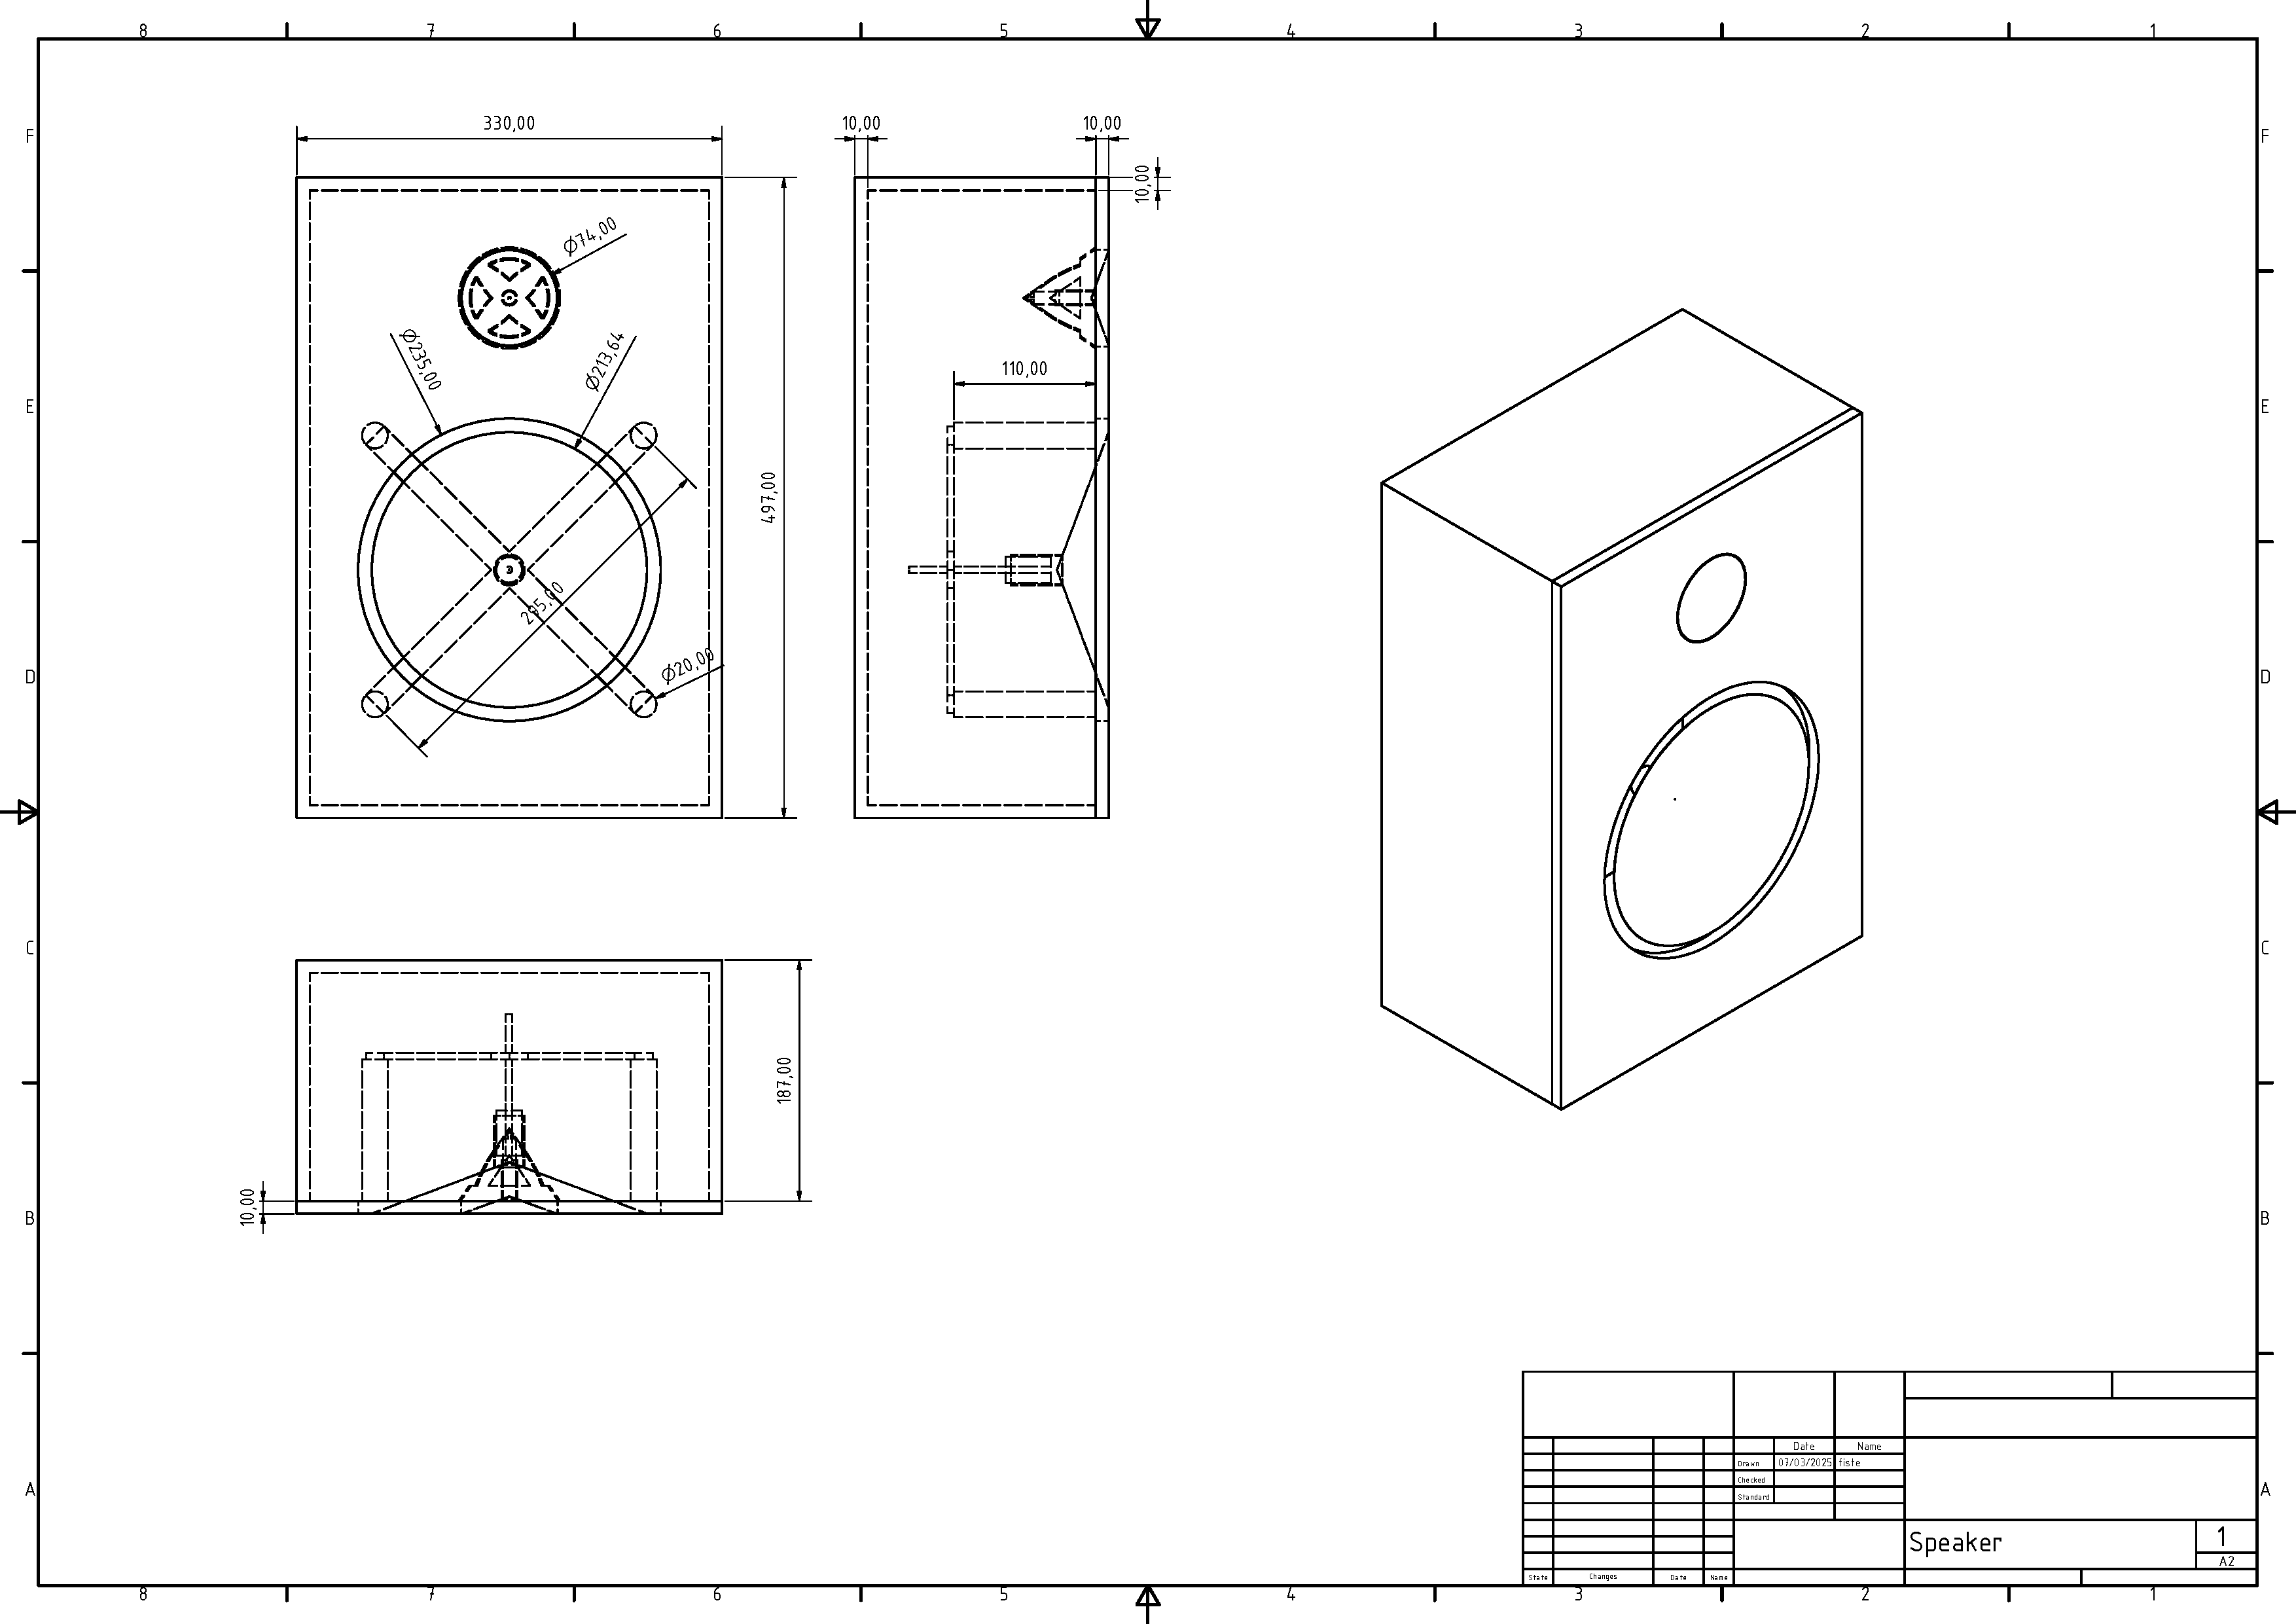
\includegraphics[width=1\textwidth]{resources/pdf/Speaker.pdf}
% How it was built
\chapter{Bau}
Die Bauform des Lautsprechers, welcher im Rahmen dieses Projektes entwickelt wurde hebt sich, speziell in seiner Komplexität, von herkömmlichen Resultaten in einem solchen Projekt ab. 
\section{Benötigte Materialien}
\begin{multicols}{2}
    \begin{itemize}[parsep=0pt]
        \item Weinkiste
        \item Deckplatte mit 235mm und 75mm Loch
        \item 9x Gewindeeinsätze M4
        \item 8x Maschinenschrauben M4 (versch. Längen)
        \item 3x Aluminiummuttern M4
        \item 5x Unterlegscheibe M4
        \item Tesa Dichtungsband 10mm
        \item Holzfaser- und Reparaturspachtel
        \item 2x Holzleisten Länge: 295mm
        \item 4x Rundstab Fichte Länge: 110mm
        \item 4x Holzschrauben Länge: 35mm
        \item Aluminium-Rundstab Durchmesser: 4,5mm
        \item Neodymmagneten mit Loch Durchmesser: 20mm
        \item Schleifpapier P180
        \item Kupferdraht Durchmeser 0,2mm
        \item Dünne Graupappe
        \item Dünner Wellkarton
        \item Neodymmagneten Durchmesser 7mm
        \item Dickes Papier
        \item Plastikröhrchen
        \item Heisskleber
        \item Hochpassfiltermodul mit Widerstand für Hochtöner
        \item Litze
        \item 2x Bananenbuchse
        \item Holzleim Rapid
        \item Isolierband
        \item Ofenschnurkleber (1100\textdegree C)
        \item Araldite Crystal
        \item Werkzeuge des Physiklbaors
    \end{itemize}
\end{multicols}

\newpage
\section{Bauanleitung}
\subsection{Gehäuse}
\begin{enumerate}
    \item Eine Weinkiste wird als Gehäuse für den Lautsprecher selbst verwendet. Um die Deckplatte zu befestigen werden Gewindeeinsätze in die Kistenwand eingebaut und Löcher in die Deckplatte gebohrt, so dass diese auf die Kiste geschraubt werden kann.
    \item Zwischen die Deckplatte und die Weinkiste wird ein Dichtungsband zur Schallabdichtung angebracht.
    \item Die Kiste wird zudem allgemein an undichten Stellen mit Holzfaser- und Reparaturspachtel abgedichtet. (Siehe Abbildung 6.1)
\end{enumerate}
\begin{figure}[h]
    \centering
    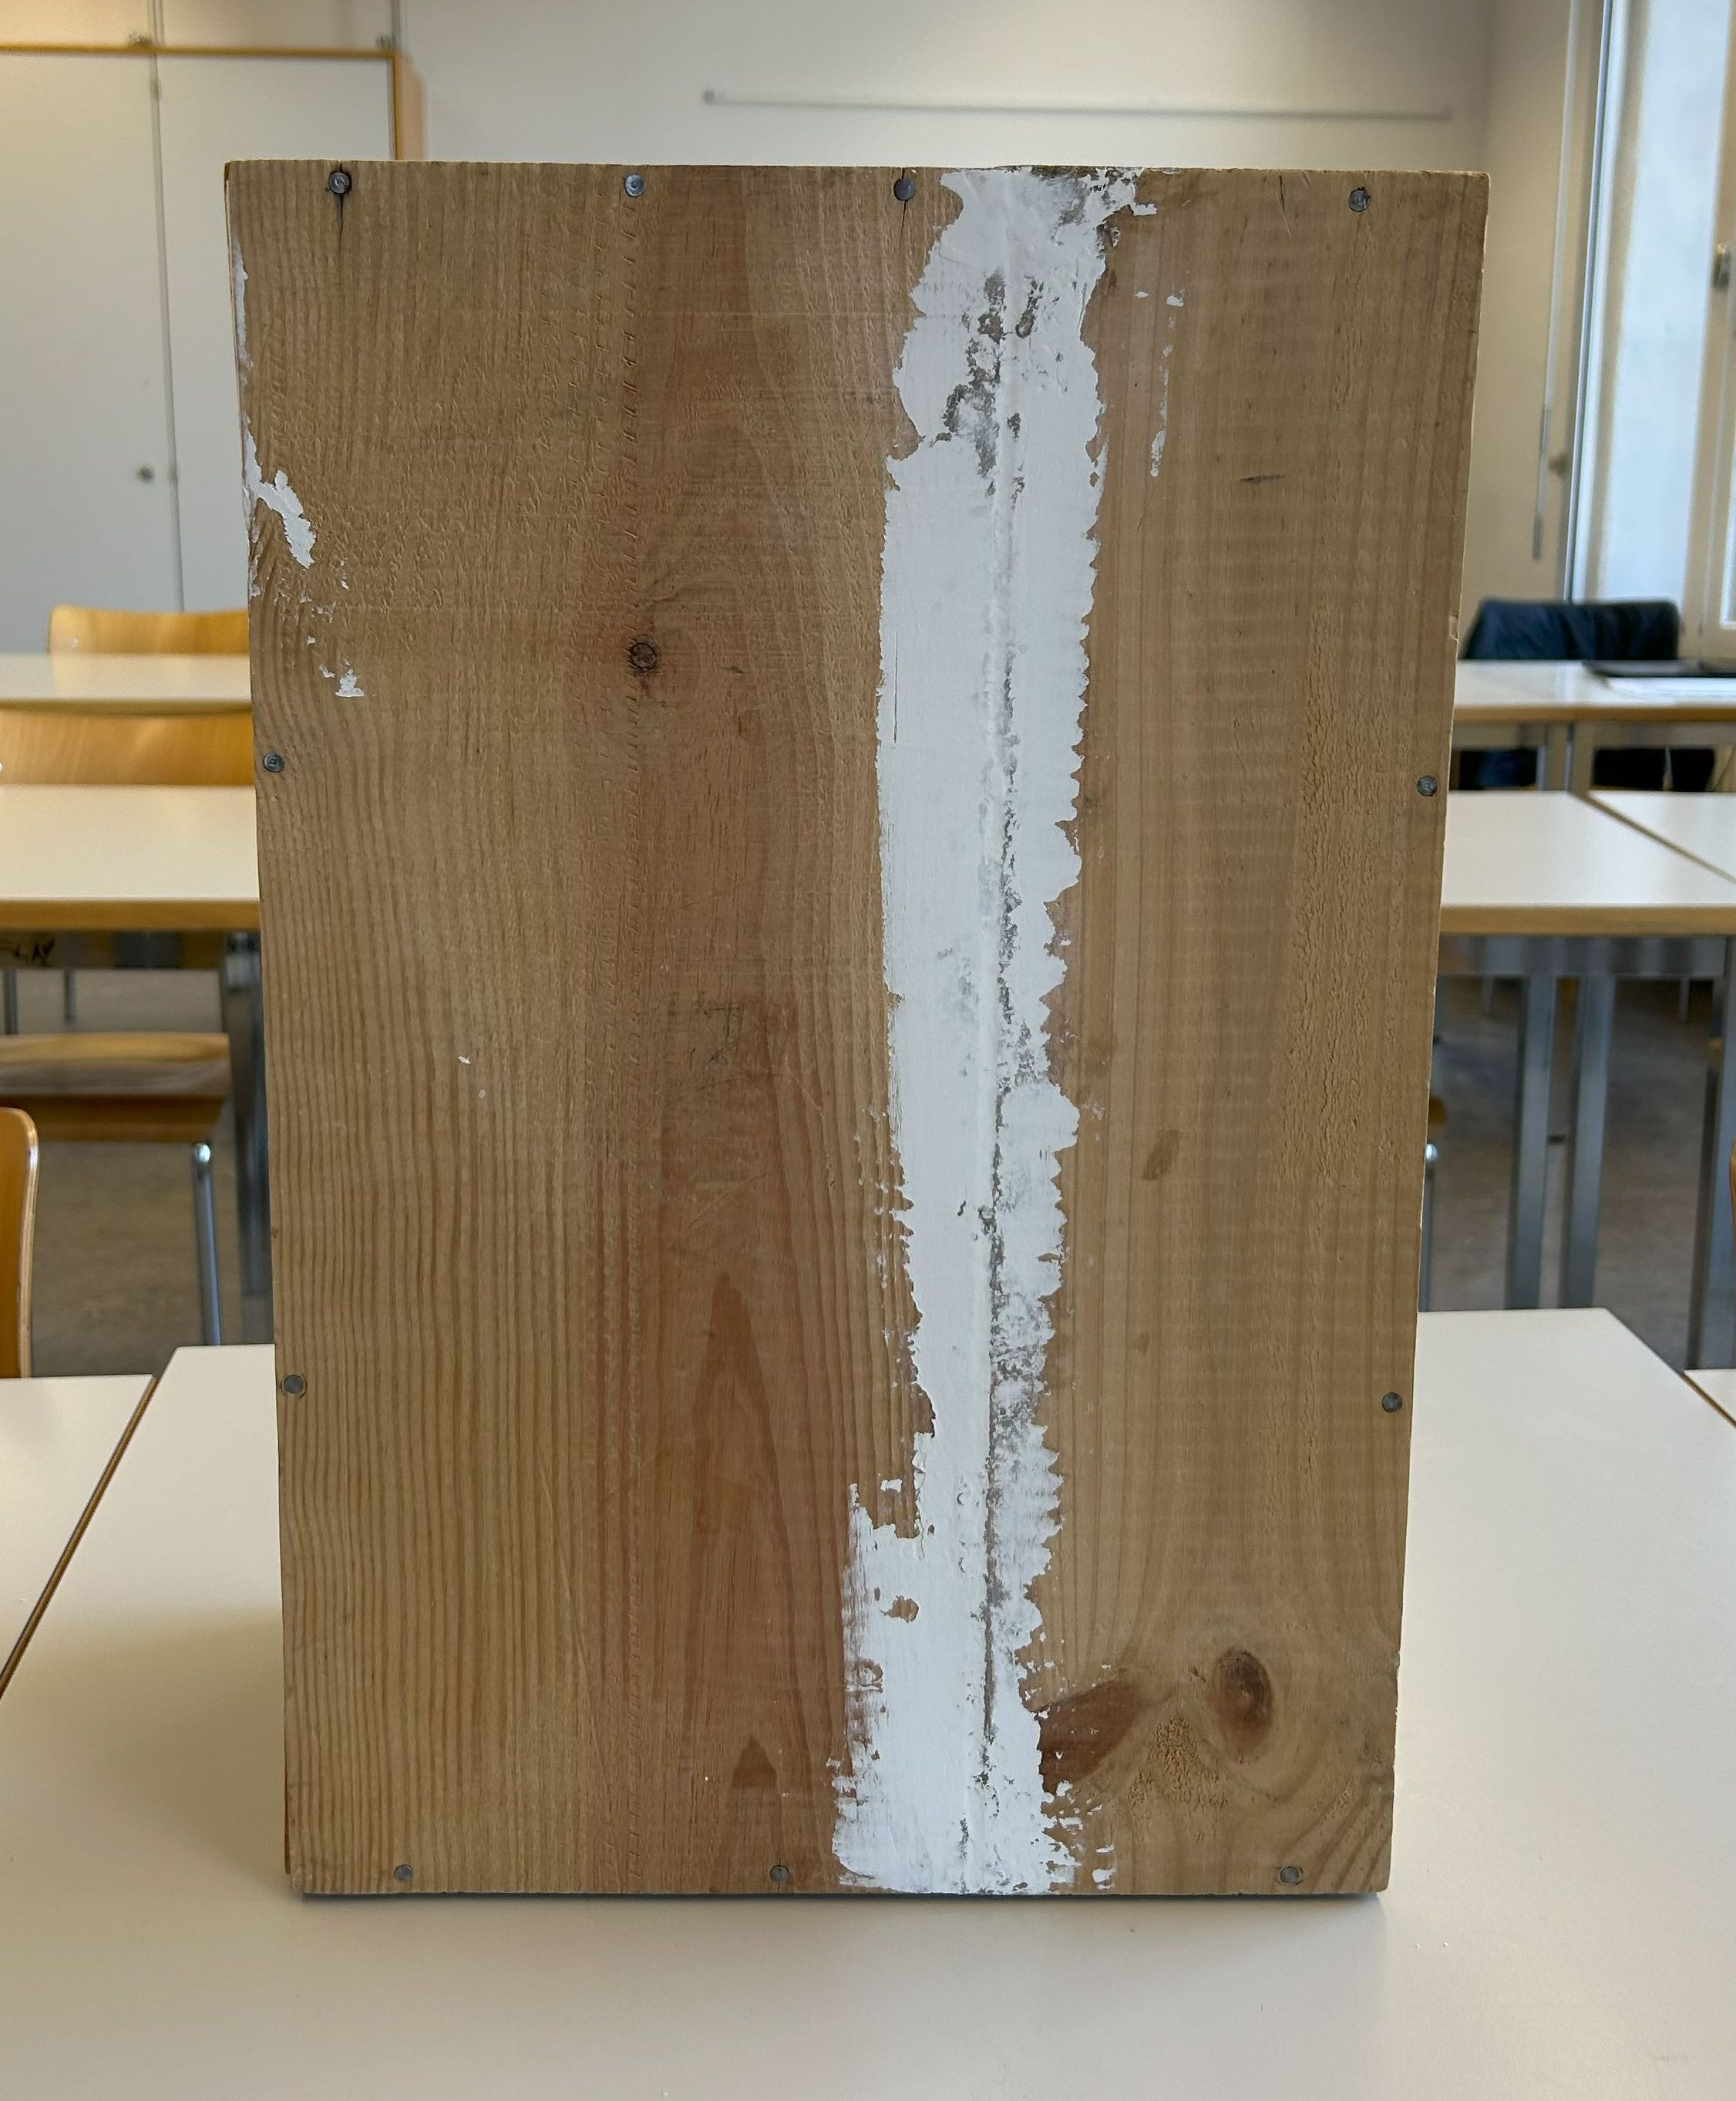
\includegraphics[width=0.5\textwidth]{resources/images/Fotos/Physik-134.jpg}
    \caption{{Abgedichtetes Gehäuse}}
    \label{fig:sealed}
\end{figure}

\newpage
\subsection{Tieftönergestell}
\begin{enumerate}
    \item Es wird zuerst ein Kreuz aus den zwei Holzleisten gebaut, mit Holzleim verleimt und in der Mitte ein Gewindeeinsatz eingelassen. (Siehe Abbildung 6.2)
    \item In die vier Rundstäbe werden von oben Gewindeeinsätze eingebaut. Sie selbst werden von hinten auf die Deckplatte geleimt und von vorne und zusätzlich mit Holzschrauben gesichert.
    \item Nun wird eine Magnet-Stelleinheit gebaut:
    \begin{enumerate}
        \item Mit einem Gewindeschneider wird ein M4 Gewinde auf die komplette Länge des Aluminium-Rundstabes geschnitten.
        \item Isoband wird zur Schwingungsisolierung der Magnete verwendet.
        \item Mit Locite und Aluminiummuttern werden die Magneten in ihrer Position fixiert.
        \item Der Aluminiumstab wird von unten in die Mitte des Holzkreuzes geschraubt und mit einer weiteren Aluminiummutter und einer Unterlegscheibe fixiert.
    \end{enumerate}
\end{enumerate}
\begin{figure}[h]
    \centering
    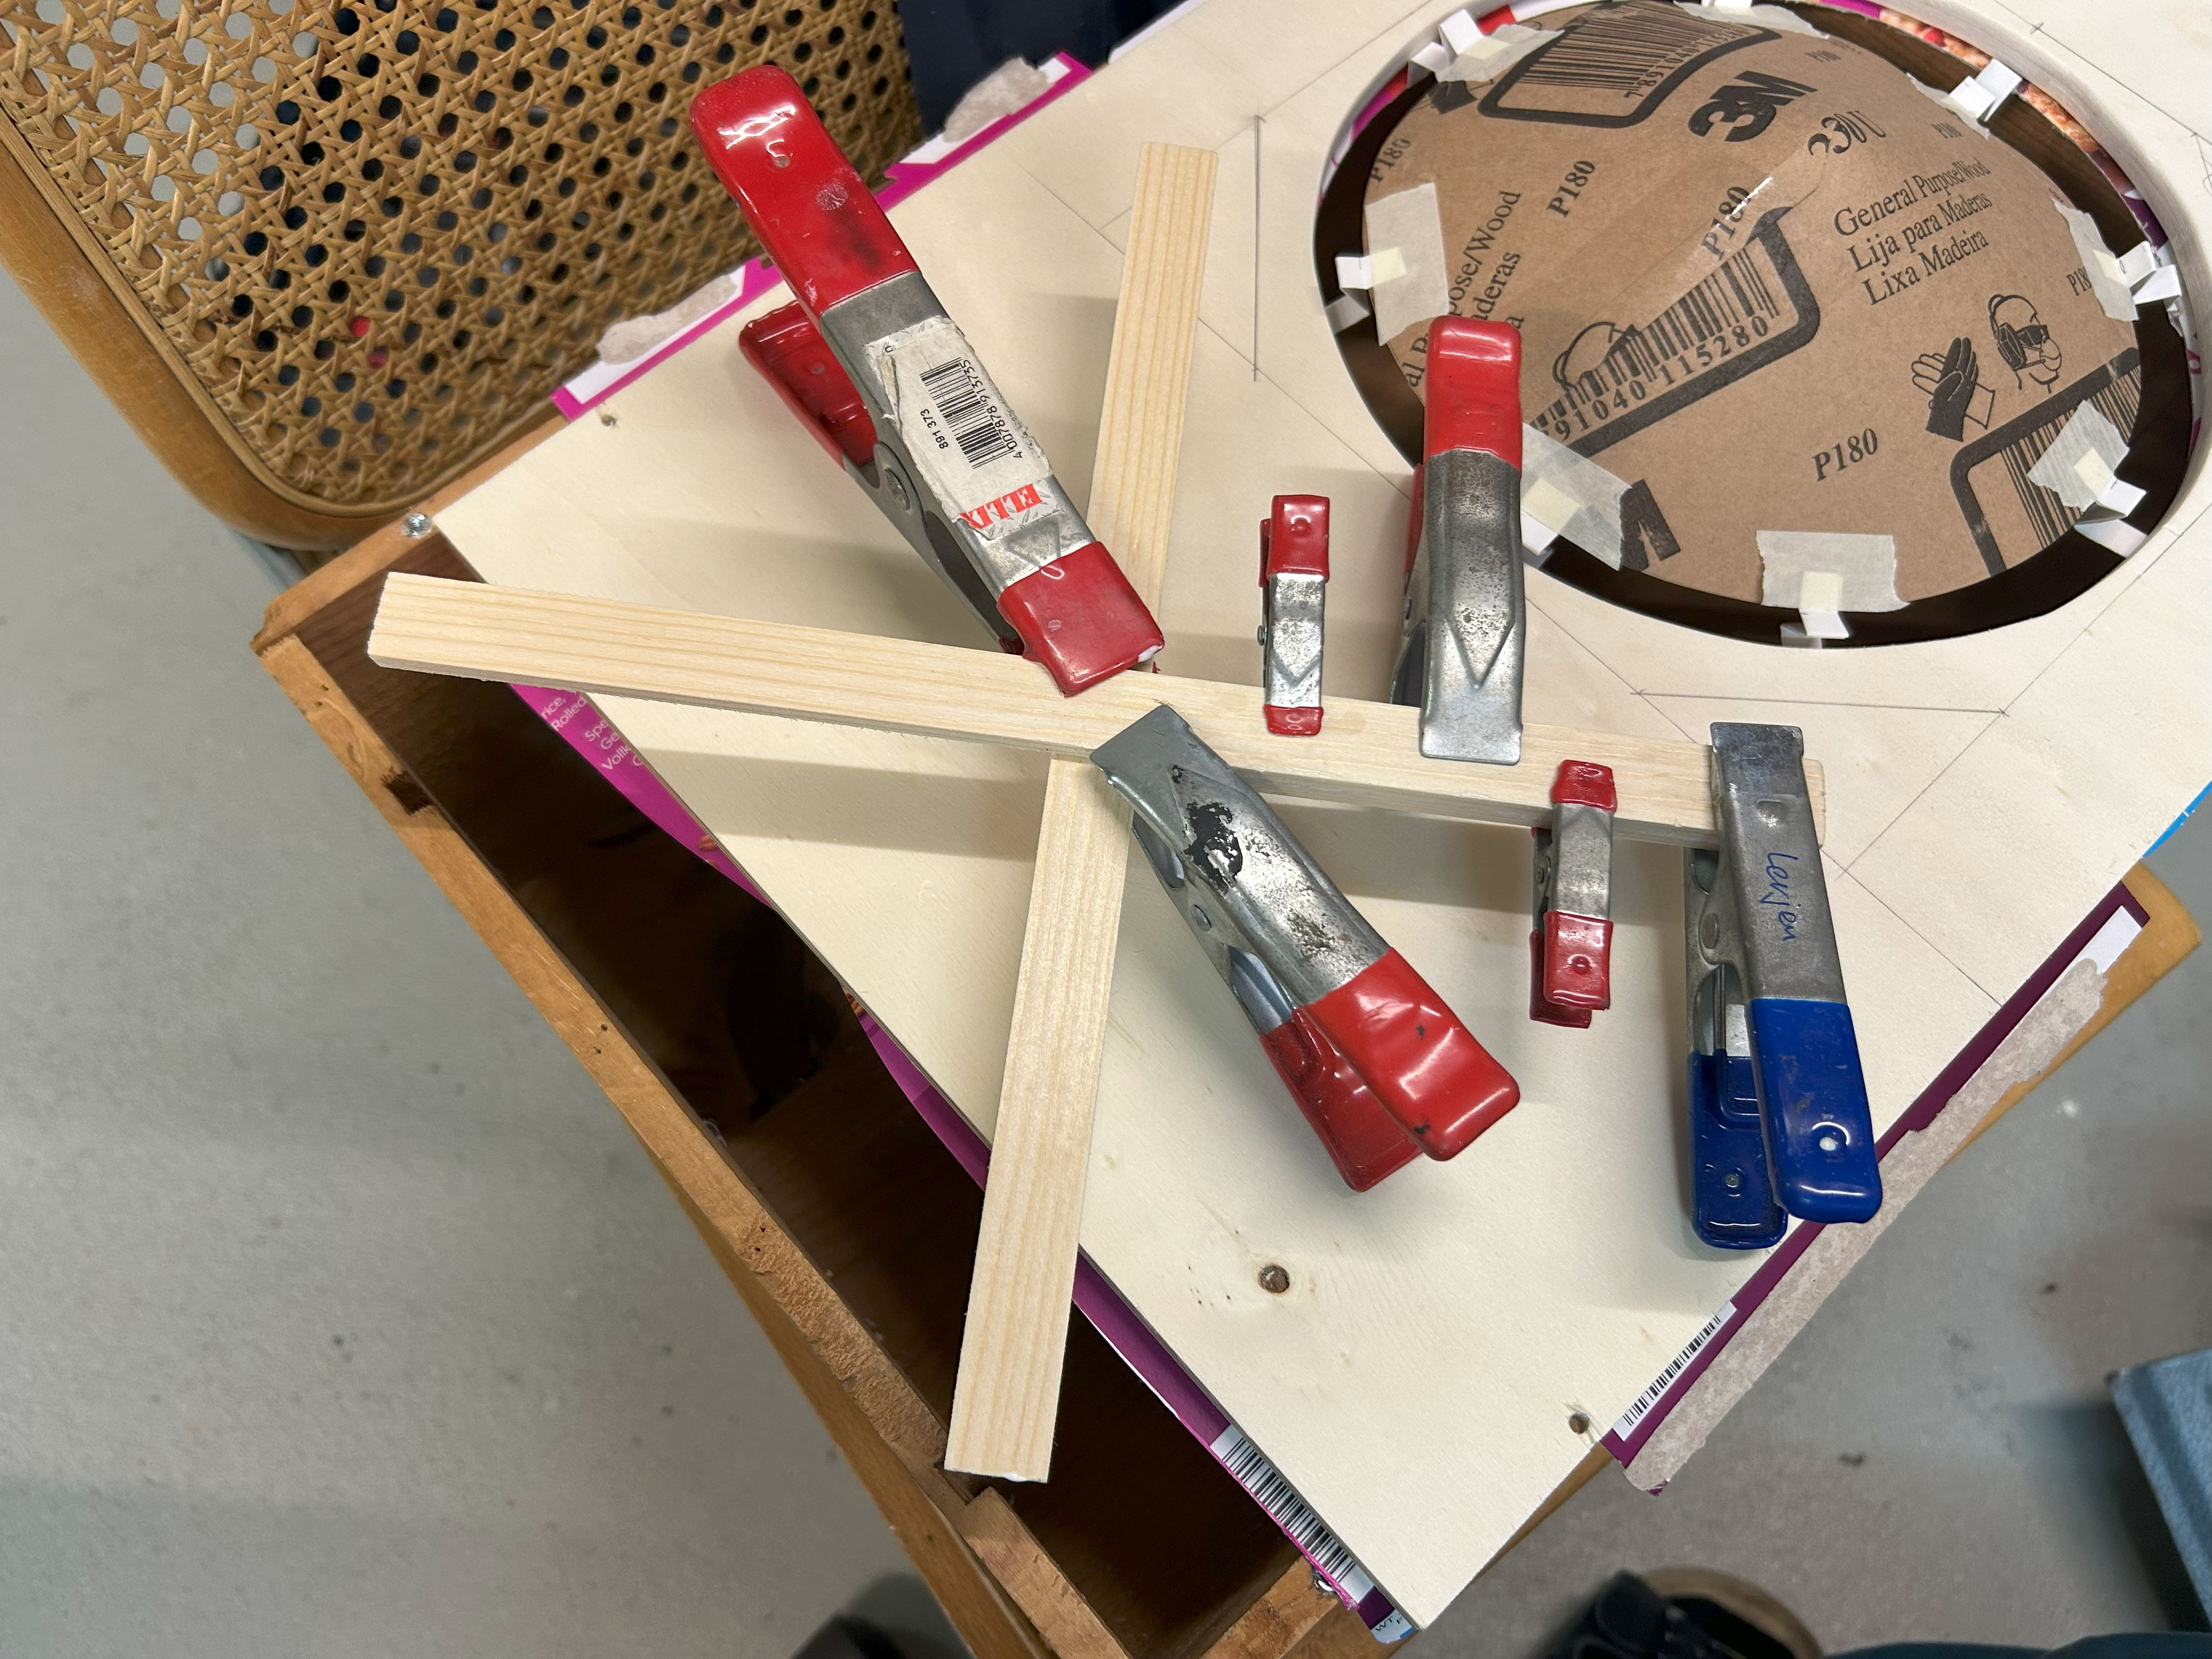
\includegraphics[width=0.5\textwidth]{resources/images/Fotos/Physik-69.jpg}
    \caption{{Tieftönergestell in Herstellung}}
    \label{fig:production}
\end{figure}

\newpage
\subsection{Tieftöner}
\begin{enumerate}
    \item Aus Schleifpapier wird eine Membran für den Tieftöner ausgeschnitten und in Kegelform zusammengeklebt, so dass dessen Grundfläche einen Durchmesser von 213mm hat und die Kegelhöhe 50mm beträgt.
    \item Aus Graupappe wird in Zylinderform der Träger für die Spule gebaut und mit Ofenschnurkleber zusammengeklebt. Um diesen Träger wird der Kupferdraht gewickelt (400 Wicklungen) und jede Schicht mit vier Streifen Ofenschnurkleber (90\textdegree versetzt) fixiert. (Siehe Abbildung 6.3)
    \item Die Spule wird anschliessend mit der Membran durch Araldite Crystal verklebt.
    \item Die C-Sicken-Streifen (Typ II) werden gefaltet und mit Isolierband verstärkt. Diese werden dann mit Holzleim immer um 45\textdegree\ versetzt an die Membran geklebt.
    \item Nun wird die Membran durch die Sickenstreifen an die Holzplatte angeleimt.
    \item Schlussendlich wird das Holzkreuz durch vier Schrauben mit vier Unterlegscheiben auf die vier Rundstäbe geschraubt. 
\end{enumerate}
\begin{figure}[h]
    \centering
    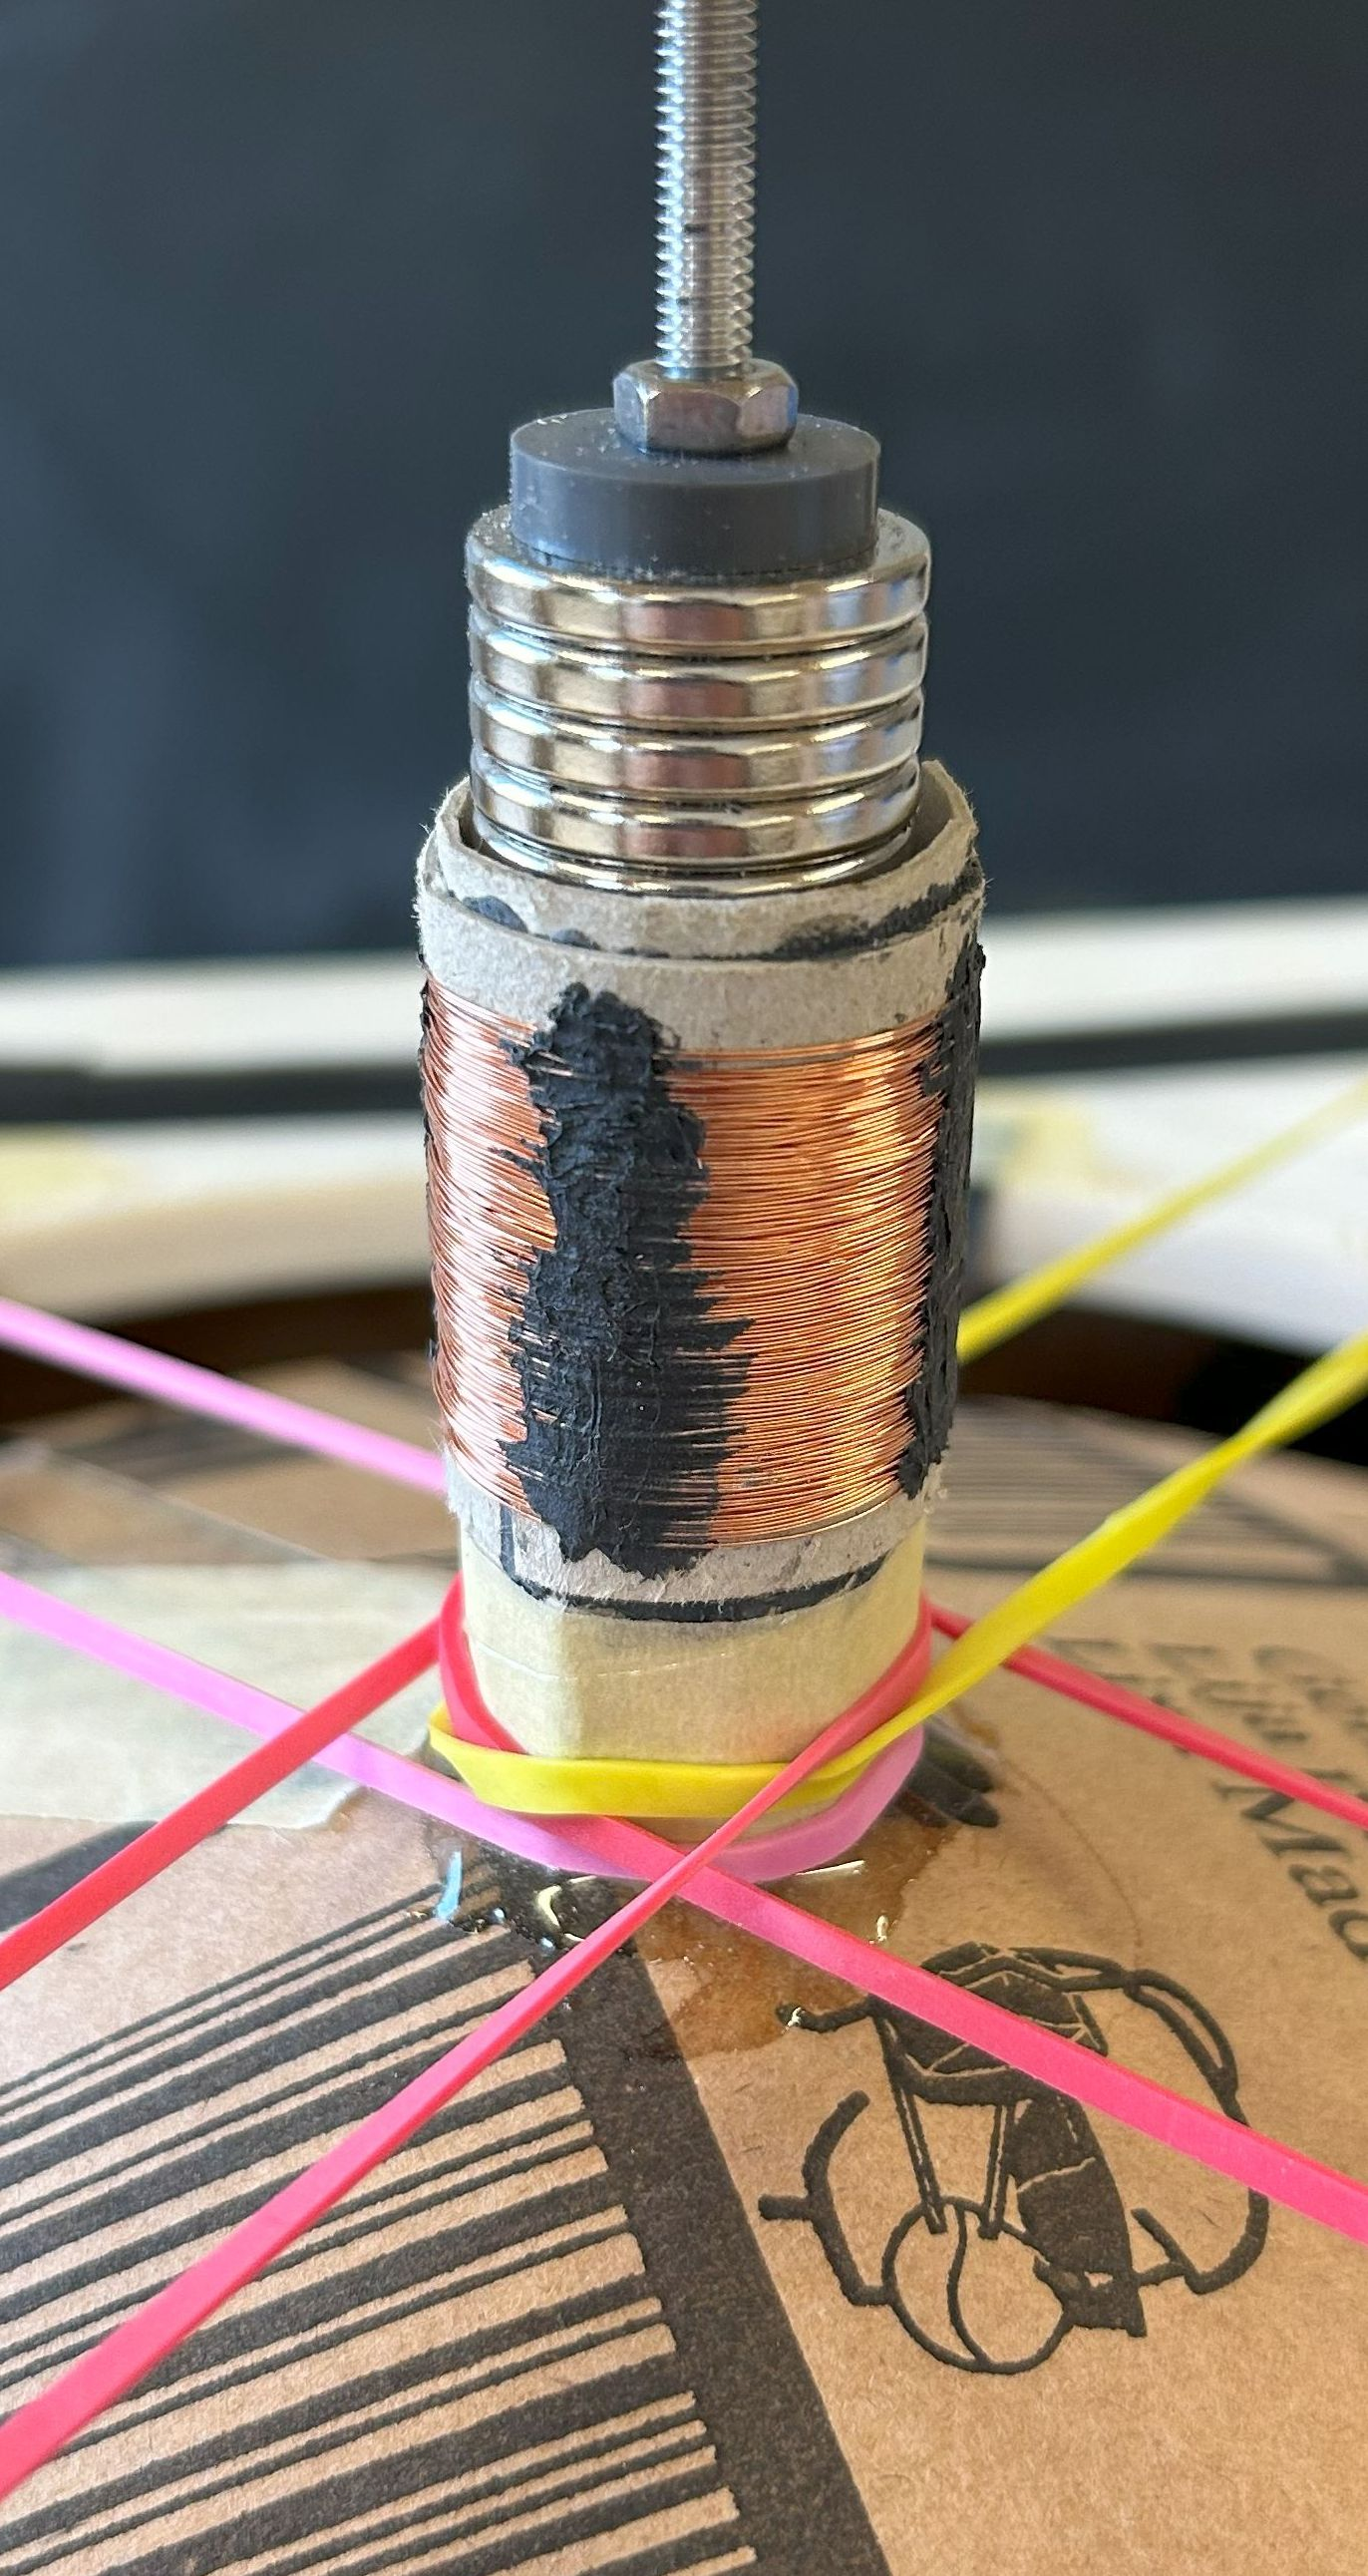
\includegraphics[width=0.3\textwidth]{resources/images/Fotos/Physik-125.jpg}
    \caption{{Fertiger Spule}}
    \label{fig:spule_fin}
\end{figure}

\newpage
\subsection{Hochtöner}
\begin{enumerate}
    \item Aus dem Wellkartonkarton wird ein kegelförmiges Gestell gebaut, welches vier Löcher in Form von Dreiecken aufweist. Die Kegelhöhe soll 80mm betragen und der Druchmesser der Grundfläche 75mm.
    \item Mithife von Araldite Crystal werden die kleinen Neodynmagnete von innen in der Kegelspitze angebracht.
    \item Eine zweite Membran wird aus Schleifpapier gebaut. Der Kegel soll eine Höhe von 10mm und die Grundfläche einen Durchmesser von 74mm aufweisen.
    \item Die zweite Spule wird mit 200 Wicklungen um einen Träger aus dickem Papier gewickelt und ebenfalls mit Ofenschnurkleber in zwei Strichen fixiert. Die Spule wird dann  Araldite Crystal an die Membran geklebt. (Siehe Abbildung 6.4)
    \item Als Sicke werden hier vier kurze Plastikröhrchen-Stücke verwendet, welche mit Heisskleber an die Membran geklebt werden.
    \item Die Membran wird über diese Sicken nun an die Gestellkonstruktion geklebt.
    \item Die Hochtönereinheit wird nun ind das kleinere Loch der Deckplatte geklebt. (Siehe Abbildung 6.5)
\end{enumerate}

\begin{minipage}{0.5\textwidth}
    \centering
    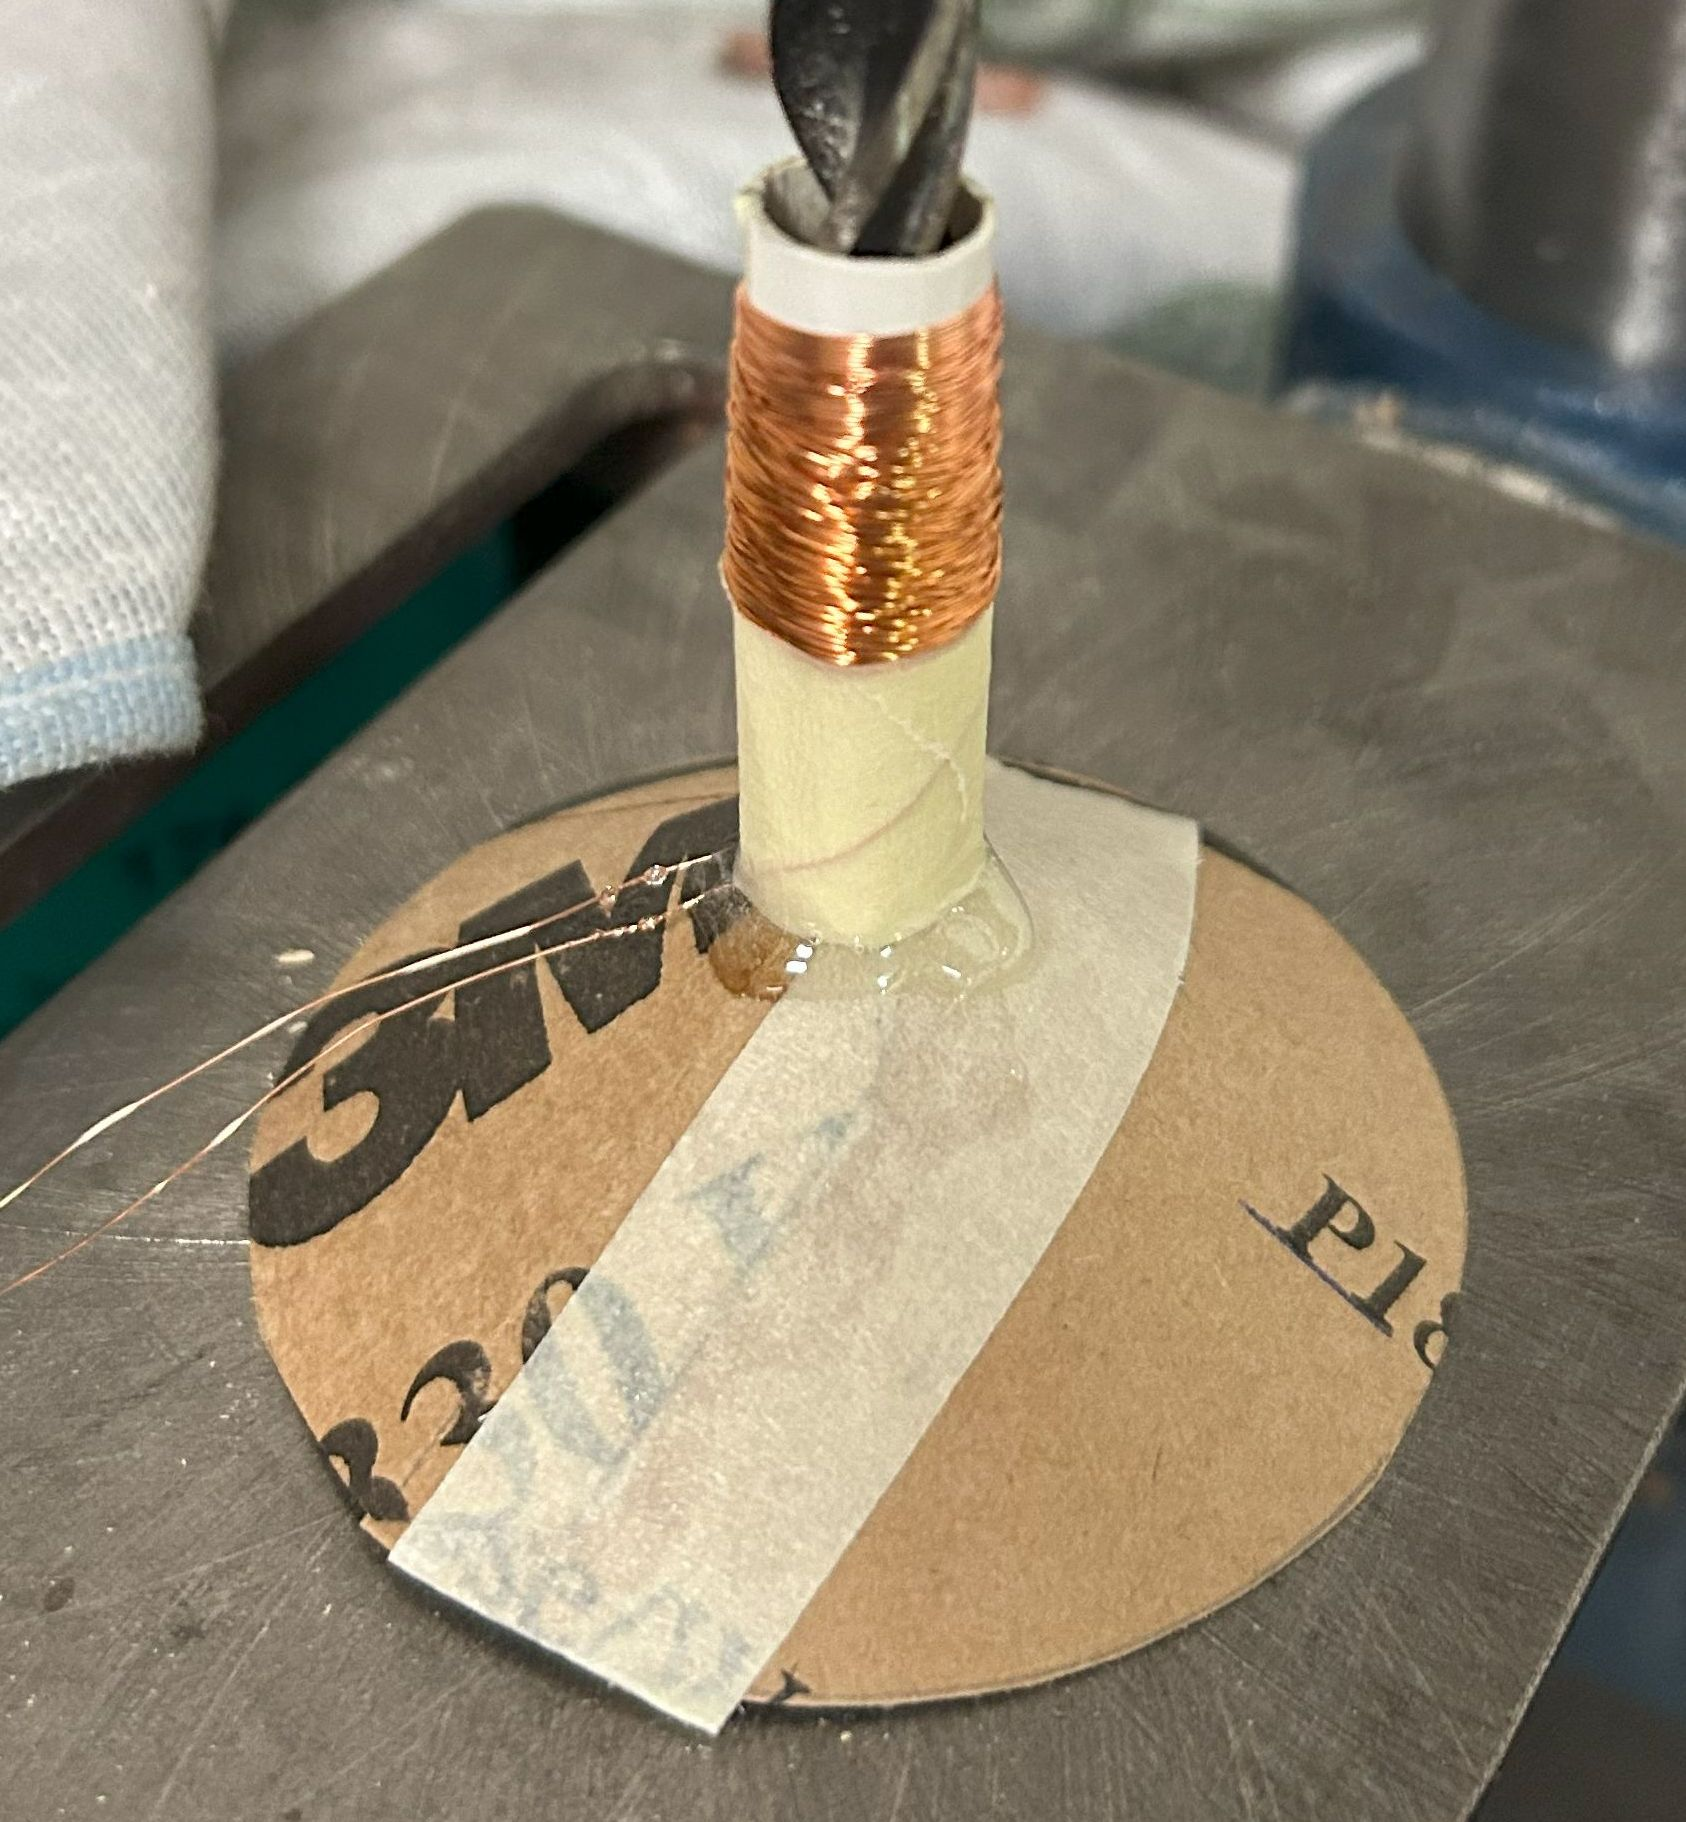
\includegraphics[width=.8\linewidth]{resources/images/Fotos/Physik-84.jpg}
    \captionof{figure}{{Fertige Hochtönermembran}}
    \label{fig:fin_high}
\end{minipage}
\begin{minipage}{0.5\textwidth}
    \centering
    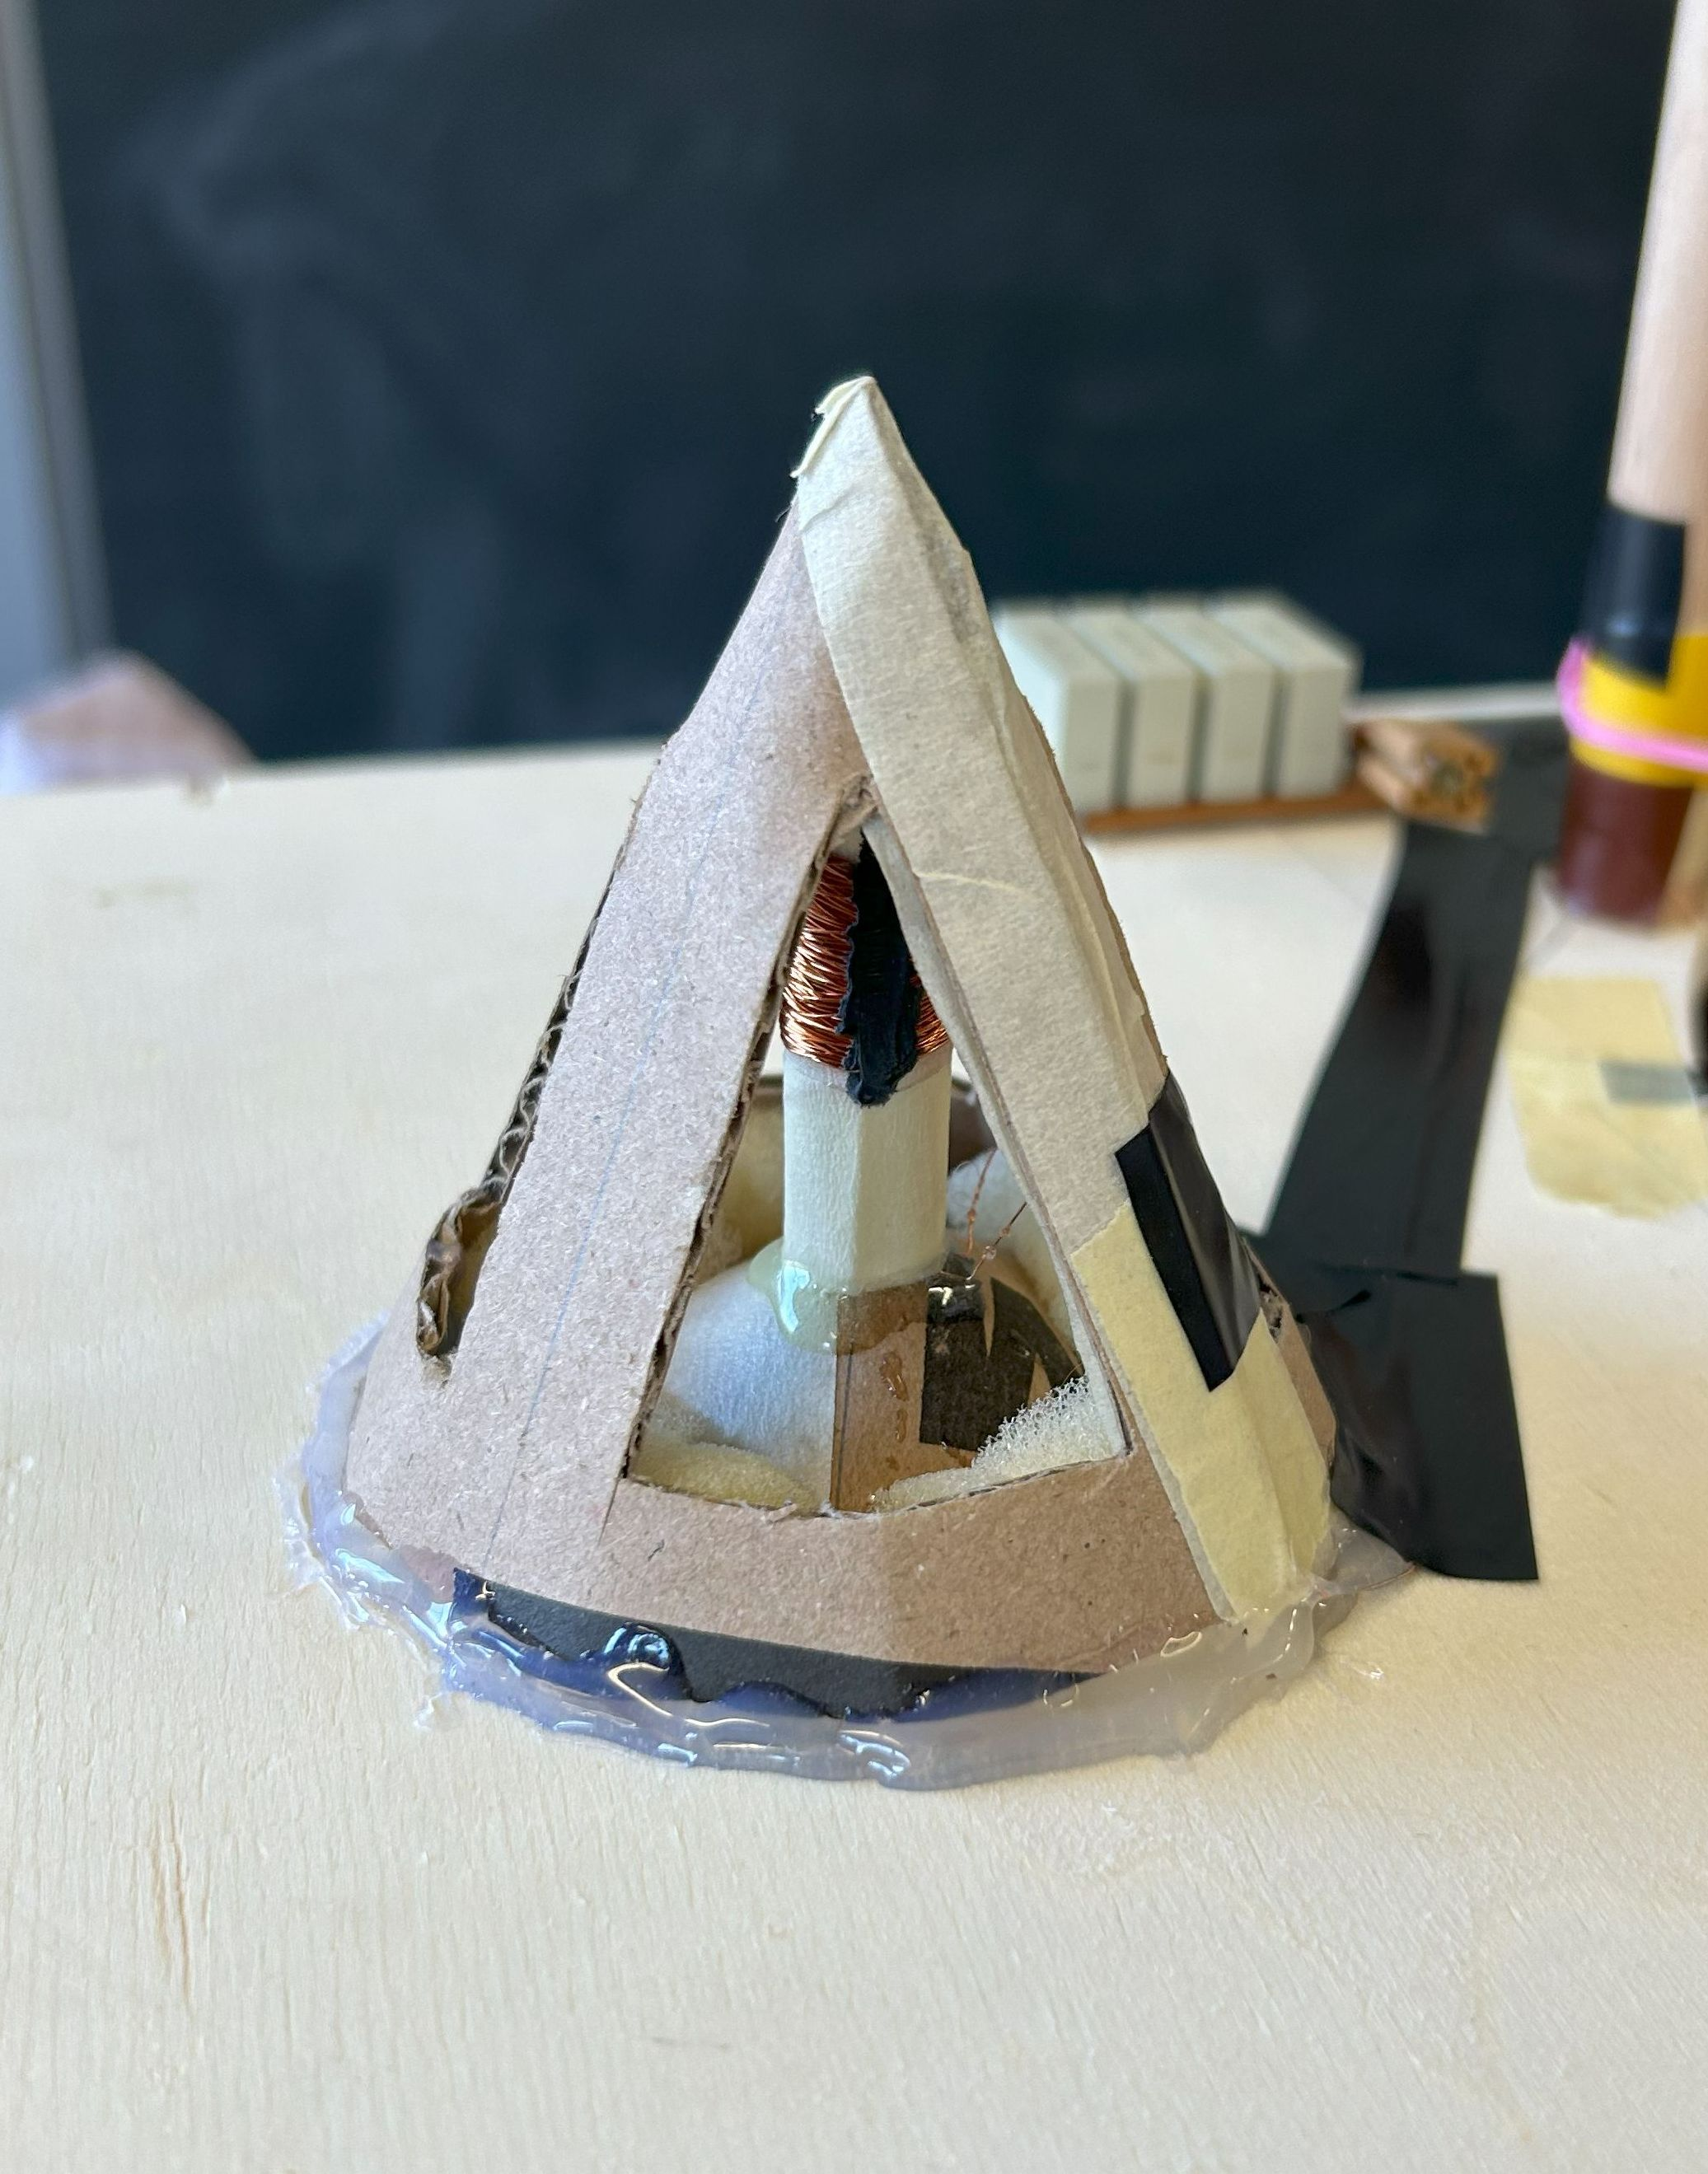
\includegraphics[width=.8\linewidth]{resources/images/Fotos/Physik-124.jpg}
    \captionof{figure}{{Fertige Hochtönereinheit}}
    \label{fig:fin_high_unit}
\end{minipage}

\newpage
\subsection{Elektrik}
\begin{enumerate}
    \item Nun müssen alle Kabel an einen zentralen Ort für das Hochpassfiltermodul verlegt werden. Dafür werden diese über ihre gesamte Länge mit Isolierband auf die Platte geklebt. Wichtig ist dabei, dass diese auch beim Übergang von Membran zur Platte über keine Kante vibrieren können sondern locker in der Luft hängen.
    \item Nun können die Kabel mit dem Hochpassfiltermodul verlötet werden. Zusätzlich werden zwei Litzenstücke an die Plattine gelötet.
    \item Es werden zwei Bananenbuchsen in der Deckplatte versenkt und die Litzen daran befestigt. Diese werden dann auch an der Platte befestigt. (Siehe Abbildung 6.6)
    \item Nun kann das Filtermodul mit Heisskleber an der Platte fixiert und die Platte auf die Weinkiste montiert werden. Der Lautsprecher kann nun verwendet werden. 
\end{enumerate}
\begin{figure}[h]
    \centering
    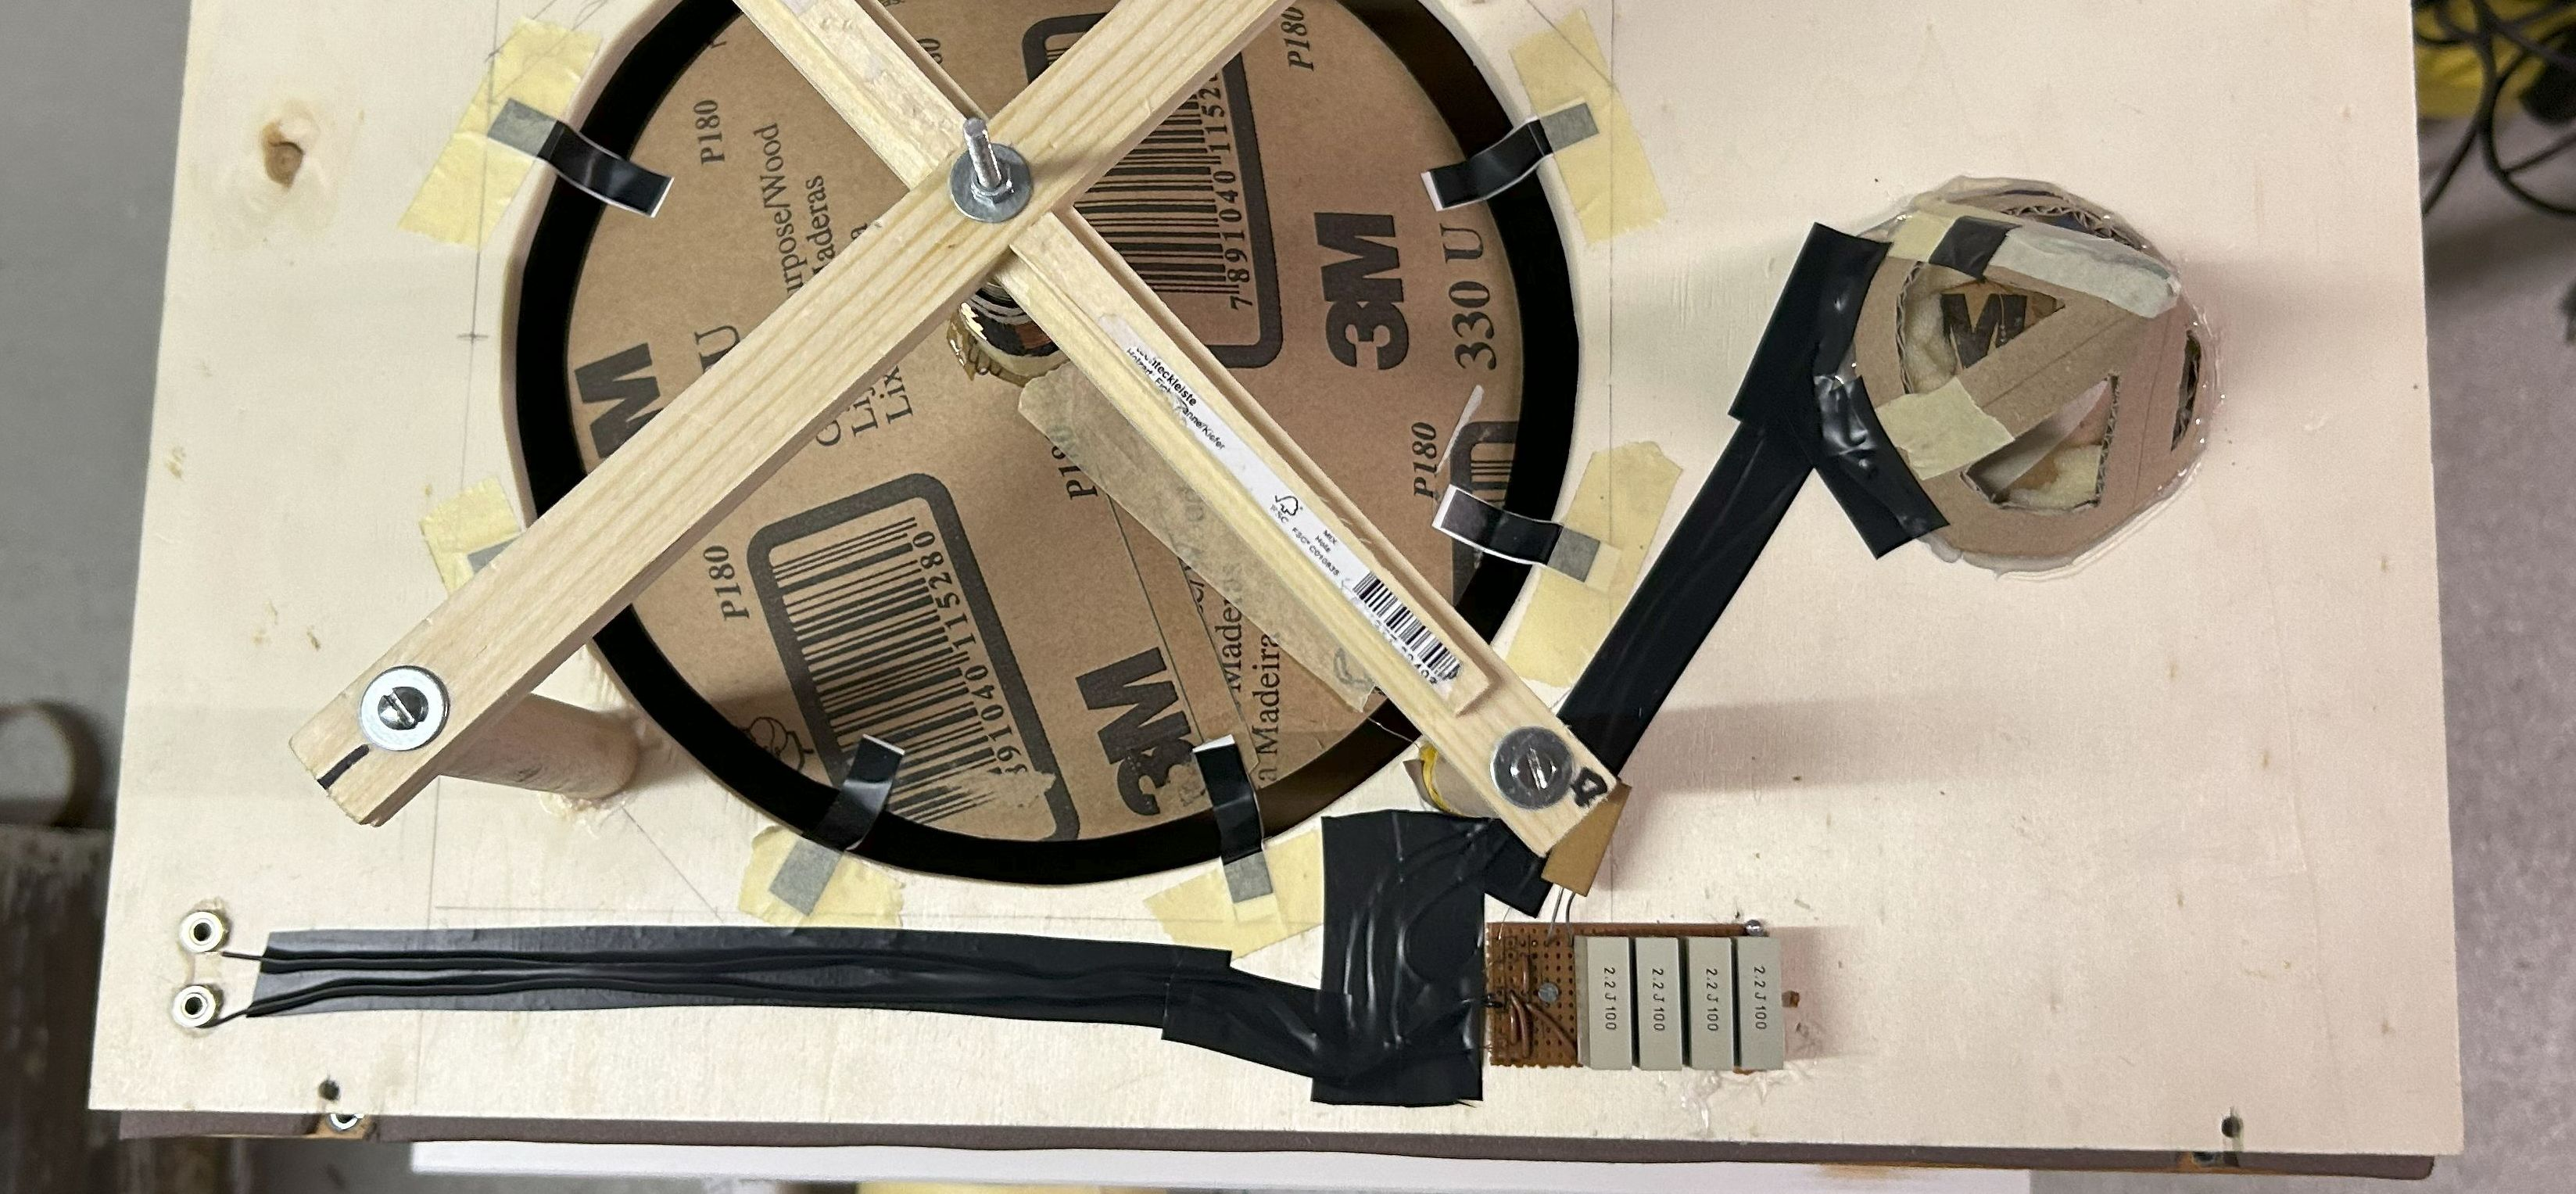
\includegraphics[width=0.7\textwidth]{resources/images/Fotos/Physik-118.jpg}
    \caption{{Verklebte Elektrik}}
    \label{fig:glued_elek}
\end{figure}
% Tanking
\chapter*{Dank}
Ein grosser Dank geht an den Physiklehrer Patrick Perucchi, welcher uns regelmässig mit Tipps und Tricks zur optimierung der Bauweise unterstützt hat.
Ein weiterer Dank geht an Herrn Daniel Meyer, welcher uns bei den Berechnungen der Frequenzweiche mit seiner Erfahrung unterstützen konnte, sowie an Markus Lerjen, welcher uns bei der Optimierung derer unterstützt hat.

Ebenfalls bedanken wir uns beim Pyhsiklaboranten und Sprengmeister Herrn Mohammed Zumsteg, welcher uns in der Werkstatt stehts zur Seite stand, uns einen Teil der Materialien und Werkzeuge zur Verfügung stelle und immer gute Sprüche geklopft hat.

% List of figures
\newpage
\listoffigures

% Sources
\newpage
\bibliographystyle{plain}
\bibliography{mybib}
\end{document}